%% abtex2-modelo-trabalho-academico.tex, v-1.9.2 laurocesar
%% Copyright 2012-2014 by abnTeX2 group at http://abntex2.googlecode.com/ 
%%
%% This work may be distributed and/or modified under the
%% conditions of the LaTeX Project Public License, either version 1.3
%% of this license or (at your option) any later version.
%% The latest version of this license is in
%%   http://www.latex-project.org/lppl.txt
%% and version 1.3 or later is part of all distributions of LaTeX
%% version 2005/12/01 or later.
%%
%% This work has the LPPL maintenance status `maintained'.
%% 
%% The Current Maintainer of this work is the abnTeX2 team, led
%% by Lauro César Araujo. Further information are available on 
%% http://abntex2.googlecode.com/
%%
%% This work consists of the files abntex2-modelo-trabalho-academico.tex,
%% abntex2-modelo-include-comandos and abntex2-modelo-references.bib
%%

% ------------------------------------------------------------------------
% ------------------------------------------------------------------------
% abnTeX2: Modelo de Trabalho Academico (tese de doutorado, dissertacao de
% mestrado e trabalhos monograficos em geral) em conformidade com 
% ABNT NBR 14724:2011: Informacao e documentacao - Trabalhos academicos -
% Apresentacao
% ------------------------------------------------------------------------
% ------------------------------------------------------------------------

\documentclass[
	% -- opções da classe memoir --
	12pt,				% tamanho da fonte
	openright,			% capítulos começam em pág ímpar (insere página vazia caso preciso)
	twoside,			% para impressão em verso e anverso. Oposto a oneside 
	% oneside twoside twoside openright openany onecolumn twocolumn
	a4paper,			% tamanho do papel. 
	% -- opções da classe abntex2 --
	%chapter=TITLE,		% títulos de capítulos convertidos em letras maiúsculas
	%section=TITLE,		% títulos de seções convertidos em letras maiúsculas
	%subsection=TITLE,	% títulos de subseções convertidos em letras maiúsculas
	%subsubsection=TITLE,% títulos de subsubseções convertidos em letras maiúsculas
	% -- opções do pacote babel --
	english,			% idioma adicional para hifenização
	french,				% idioma adicional para hifenização
	spanish,			% idioma adicional para hifenização
	brazil				% o último idioma é o principal do documento
	]{abntex2}

% ---
% Pacotes básicos 
% ---
\usepackage{lmodern}			% Usa a fonte Latin Modern			
\usepackage[T1]{fontenc}		% Selecao de codigos de fonte.
\usepackage[utf8]{inputenc}		% Codificacao do documento (conversão automática dos acentos)
\usepackage{lastpage}			% Usado pela Ficha catalográfica
\usepackage{indentfirst}		% Indenta o primeiro parágrafo de cada seção.
\usepackage{color}				% Controle das cores
\usepackage{graphicx}			% Inclusão de gráficos
\usepackage{microtype} 			% para melhorias de justificação
\usepackage{array}
\usepackage[table,xcdraw]{xcolor}
% ---

%força tabelas a nao reposicionarem		
\usepackage{placeins}

%citação usando modelo autor - data

% apendice
%\usepackage[titletoc]{appendix}
%\renewcommand\cftappendixname{\appendixname~}
%\AtBeginDocument{\renewcommand\appendixname{New Name}}

%%%CODE
\usepackage{listings}
\usepackage{caption}

\lstset{literate=
  {á}{{\'a~}}1 {é}{{\'e~}}1 {í}{{\'i~}}1 {ó}{{\'o~}}1 {ú}{{\'u~}}1
  {ã}{{\~a~}}1 {ẽ}{{\~e~}}1 {ĩ}{{\~i~}}1 {õ}{{\~o~}}1 {ũ}{{\~u~}}1
  {Á}{{\'A~}}1 {É}{{\'E~}}1 {Í}{{\'I~}}1 {Ó}{{\'O~}}1 {Ú}{{\'U~}}1
  {à}{{\`a~}}1 {è}{{\`e~}}1 {ì}{{\`i~}}1 {ò}{{\`o~}}1 {ù}{{\`u~}}1
  {À}{{\`A~}}1 {È}{{\'E~}}1 {Ì}{{\`I~}}1 {Ò}{{\`O~}}1 {Ù}{{\`U~}}1
  {ä}{{\"a~}}1 {ë}{{\"e~}}1 {ï}{{\"i~}}1 {ö}{{\"o~}}1 {ü}{{\"u~}}1
  {Ä}{{\"A~}}1 {Ë}{{\"E~}}1 {Ï}{{\"I~}}1 {Ö}{{\"O~}}1 {Ü}{{\"U~}}1
  {â}{{\^a~}}1 {ê}{{\^e~}}1 {î}{{\^i~}}1 {ô}{{\^o~}}1 {û}{{\^u~}}1
  {Â}{{\^A~}}1 {Ê}{{\^E~}}1 {Î}{{\^I~}}1 {Ô}{{\^O~}}1 {Û}{{\^U~}}1
  {œ}{{\oe~}}1 {Œ}{{\OE~}}1 {æ}{{\ae~}}1 {Æ}{{\AE~}}1 {ß}{{\ss~}}1
  {ç}{{\c c~}}1 {Ç}{{\c C~}}1 {ø}{{\o~}}1 {å}{{\r a~}}1 {Å}{{\r A~}}1
  {€}{{\EUR~}}1 {£}{{\pounds~}}1
}



\definecolor{dkgreen}{rgb}{0,0.6,0}
\definecolor{gray}{rgb}{0.5,0.5,0.5}
\definecolor{mauve}{rgb}{0.58,0,0.82}

\lstset{frame=tb,
  language=bash,
  aboveskip=3mm,
  belowskip=3mm,
  showstringspaces=false,
  columns=flexible,
  basicstyle={\small\ttfamily},
  numbers=none,
  numberstyle=\tiny\color{gray},
  keywordstyle=\color{blue},
  commentstyle=\color{dkgreen},
  stringstyle=\color{mauve},
  breaklines=true,
  breakatwhitespace=true,    % added this
  tabsize=3
}
%\DeclareCaptionFormat{listing}{\rule{\dimexpr\textwidth+17pt\relax}{0.4pt}\par\vskip1pt#1#2#3}
%\captionsetup[lstlisting]{format=listing,singlelinecheck=false, margin=0pt, font={sf},labelsep=space,labelfont=bf}

\renewcommand{\lstlistingname}{Código}




% ---
% Pacotes de citações
% ---
\usepackage[alf]{abntex2cite}	% Citações padrão ABNT

% --- 
% CONFIGURAÇÕES DE PACOTES
% --- 
\usepackage[maxfloats=40]{morefloats}
\usepackage{float}
\usepackage{pdfpages}
\usepackage{amsmath}
\usepackage{multirow}
\usepackage{csquotes}
% helvetica no titulo dos capitulos
%\usepackage[scaled]{helvet}
\usepackage{tgheros}
\renewcommand{\ABNTEXchapterfont}{\fontfamily{\sfdefault}\selectfont}
\renewcommand{\ABNTEXchapterfontsize}{\HUGE}
%real numbers
\usepackage{amssymb}
%\hyphenation{Recomendação}


% ---
% Informações de dados para CAPA e FOLHA DE ROSTO
% ---
\titulo{%
Compliance\\
\large Como a operação Lava Jato trouxe mudanças na aplicação dos metodos de compliance em empresas mediante a Lei n. 12.846/2013 (Lei Anticorrupção)}
\autor{Bruna Guglielimi Pereira}
\local{São Bernardo do Campo, São Paulo}
\data{2019}
\tipotrabalho{Trabalho de Formatura}
% O preambulo deve conter o tipo do trabalho, o objetivo, 
% o nome da instituição e a área de concentração 
\preambulo{Trabalho de Conclusão de Curso apresentado à banca Examinadora da Faculdade de Direito São Bernardo do Campo, como exigência parcial para obtenção do grau de Bacharel em Direito, sob orientação do Professor - Orientador Dr. Ezio Carlos Silva Baptista} 
% ---
\DeclareMathOperator*{\argmax}{arg\,max}

 
% ---
% Configurações de aparência do PDF final

% alterando o aspecto da cor azul
\definecolor{blue}{RGB}{41,5,195}

% informações do PDF
\makeatletter
\hypersetup{
     	%pagebackref=true,
		pdftitle={\@title}, 
		pdfauthor={\@author},
    	pdfsubject={\imprimirpreambulo},
	    pdfcreator={LaTeX with abnTeX2},
		pdfkeywords={startup}{lean}{beacons}{mobile advertising}{trabalho acadêmico}{varejo}, 
		colorlinks=true,       		% false: boxed links; true: colored links
    	linkcolor=blue,          	% color of internal links
    	citecolor=blue,        		% color of links to bibliography
    	filecolor=magenta,      		% color of file links
		urlcolor=blue,
		bookmarksdepth=4
}
\makeatother
% --- 

% --- 
% Espaçamentos entre linhas e parágrafos 
% --- 

% O tamanho do parágrafo é dado por:
\setlength{\parindent}{1.3cm}

% Controle do espaçamento entre um parágrafo e outro:
\setlength{\parskip}{0.2cm}  % tente também \onelineskip

% ---
% compila o indice
% ---
\makeindex
% ---

% ----
% Início do documento
% ----
\begin{document}

% Retira espaço extra obsoleto entre as frases.
\frenchspacing 

% ----------------------------------------------------------
% ELEMENTOS PRÉ-TEXTUAIS
% ----------------------------------------------------------
% \pretextual

\imprimircapa

\imprimirfolhaderosto %falsa folha de rosto

\orientador{Prof. Dr. Ezio Carlos Silva Baptista}

\imprimirfolhaderosto*

%!TEX root = index.tex
\begin{fichacatalografica}\label{ficha catalografica}
	\vspace*{\fill}					% Posição vertical
	\hrule							% Linha horizontal
	\begin{center}					% Minipage Centralizado
	\begin{minipage}[c]{12.5cm}		% Largura
	
	\imprimirautor
	
	\hspace{0.5cm} \imprimirtitulo  / C. E. U Saiki. --
	\imprimirlocal, \imprimirdata
	
	\hspace{0.5cm} \pageref{LastPage} p.\\
	
	\hspace{0.5cm} \imprimirorientadorRotulo~\imprimirorientador\\
	
	\hspace{0.5cm}
	\parbox[t]{\textwidth}{\imprimirtipotrabalho~--~Escola Politécnica da Universidade de São Paulo. Departamento de Engenharia de Produção.}\\
	
	\hspace{0.5cm}
		%1. Startup.
		%2. Lean.
		%3. Beacons.
		%4. Varejo
		I. Prof. Dr. André Leme Fleury.
		II. Universidade de São Paulo. Escola Politécnica.
		III. Departamento de Engenharia de Produção\\ 
	
	%\hspace{8.75cm} CDU xx.xxx.xxx.x\\
	
	\end{minipage}
	\end{center}
	\hrule
\end{fichacatalografica}
%\pagebreak

%\input{folha_de_aprovacao}
%\pagebreak

%%!TEX root = index.tex
\begin{dedicatoria}
   \vspace*{\fill}
   \centering
   \noindent
   \textit{ Dedico esse trabalho a minha família} \vspace*{\fill}
\end{dedicatoria}
%\pagebreak

%!TEX root = index.tex
\begin{agradecimentos}


   Primeiramente, gostaria de agradecer as pessoas que me fizeram passar de ano e me ajudaram a estudar sempre que precisei. Obrigada Emanuele e Vitor, vocês são incríveis e eu não estaria me graduando se não fosse por vocês. 

   Além disso, gostaria de agradecer minhas maravilhosas amigas que estiveram do meu lado nos melhores e piores momentos e que me incentivavam a sair cama quase todos os dias. Obrigada Brunna, Giulia, Maysa, Giovanna e Bea (mesmo que só até o 3º ano né.)

   Não menos importante, gostaria de agradecer aqueles que me deram suporte mesmo que fora da faculdade, obrigada Amanda e Christian, minha melhor amiga e meu namorado são as pessoas mais maravilhosas que sempre fizeram alguma gracinha para que eu não surtasse muito nos momentos de crise. 

   Por fim, mas definitivamente nao menos importante, agradeço minha família por me acompanhar ao fim desta jornada. Foi longa, mas ao mesmo tempo passou em um piscar de olhos. Graças a eles hoje posso dizer que me formei e posso seguir adiante. Obrigada papai, mamãe e lucas, vocês são incríveis e insubstituíveis na minha vida. 

\end{agradecimentos}

%\pagebreak

%!TEX root = index.tex
\begin{epigrafe}
    \vspace*{\fill}
	\begin{flushright}
		\textit{“Arrisque-se!}
		
		\textit{O homem que vai mais longe é geralmente}
		
		\textit{aquele que está disposto a fazer e ousar.”} 
		
		(Dale Carnegie)
	\end{flushright}
\end{epigrafe}
%\pagebreak

%!TEX root = index.tex
% resumo em português
\setlength{\absparsep}{18pt} % ajusta o espaçamento dos parágrafos do resumo
\begin{resumo}
Esse trabalho de conclusão de curso de Engenharia de Produção da Escola Politécnica da Universidade de São Paulo teve como objetivo reestruturar uma startup que teve um nascimento turbulento. Foi utilizado um método que teve como base a utilização dos princípios da Startup Enxuta, do Desenvolvimento de Clientes e do Canvas de Modelo de Negócio.

A empresa nascente desse trabalho desenvolveu um aplicativo de descontos em lojas físicas, cujo diferencial era a utilização da tecnologia de beacons para conseguir uma melhor precisão para geolocalização em ambientes internos. Assim, o aplicativo conseguiria oferecer o melhor desconto para usuário baseado na localização do mesmo. O principal desafio da empresa era crescer tanto a base de usuários quanto o número de lojas presentes no aplicativo.

O autor desse trabalho é um dos fundadores da empresa e esteve presente em todo os processos decisivos e no desenvolvimento do aplicativo. Para que o trabalho fosse desenvolvido o autor elaborou um método para que fosse possível testar as hipóteses essenciais da empresa de forma sistemática. Além disso, o método demandava que o aprendizado adquirido durante cada ciclo de testes fosse registrado para que a empresa não cometesse os mesmos erros novamente.

No primeiro ciclo de testes o objetivo foi testar se os usuários viam valor no aplicativo, se era possível conseguir novos usuários de forma barata utilizando as redes sociais e se os varejistas tinham interesse em aderir a esse novo aplicativo.

No segundo ciclo de testes o objetivo foi checar se os varejistas estavam dispostos a pagar pela utilização do serviço, dado que até o momento nenhum parceiro estava pagando pelo uso da plataforma disponibilizada pelo aplicativo, ou seja, a receita da empresa era nula.

O trabalho apresentado é o resultado de uma busca para tentar salvar uma empresa, cujo sonho era o de revolucionar o varejo físico brasileiro e um dia o do mundo.

\textbf{Palavras-chaves}: Empresa, Nascente, Enxuta, Beacons, Varejo.
\end{resumo}
%\pagebreak

%!TEX root = index.tex
% resumo em português
\setlength{\absparsep}{18pt} % ajusta o espaçamento dos parágrafos do resumo
\begin{resumo}[Abstract]
 \begin{otherlanguage*}{english}
The purpose of this undergraduate thesis of the Industrial Engineering course of the Polytechnic School of the University of São Paulo hereby presented was to restructure a startup that has had a turbulent start. The method that was applied was based on the principles of the Lean Startup, the Customer Development and the Business Model Canvas.

The startup of this thesis developed a discount app for brick-and-mortar shops, whose difference was the use of beacons technology to achieve better accuracy for geolocation indoors. Thus, the app would offer the best discount for a user based on the location of the same. The main challenge was to grow the company on both the user and the brick-and-mortar side.

The author of this thesis is one of the founders of the company and was present throughout the decision-making processes and application development. For the work to be developed the author elaborated a method to make it possible to test systematically the key assumptions of the company. In addition, the method demanded that the learning acquired during each test cycle were recorded for the company not to commit the same mistakes again.

In the first test cycle the goal was to test whether users saw value in the application, if it was possible to get new users inexpensively using social networks and if the retailers were interested in joining this new application.

In the second test cycle the goal was to see if retailers were willing to pay to use the service, as to date no partner was paying for the use of the platform provided by the application, ie, the company's revenue was nil.

The presented work is the result of a search to try to save a company, whose dream was to revolutionize the Brazilian physical retail and one day the world.

   \vspace{\onelineskip}
 
   \noindent 
   \textbf{Keywords}: Beacons, Lean, Startup, Retail.
 \end{otherlanguage*}
\end{resumo}

%\pagebreak

% inserir lista de tabelas
% ---
\pdfbookmark[0]{\listtablename}{lot}
\listoftables*
\cleardoublepage
\listoffigures*
\cleardoublepage

% inserir o sumario
\pdfbookmark[0]{\contentsname}{toc}
\tableofcontents*
\cleardoublepage
% ---

% ----------------------------------------------------------
% ELEMENTOS TEXTUAIS
% ----------------------------------------------------------
\textual


%inteligencia artificial
%aprendizado computacional
% comercio eletronico
% produtos

%!TEX root = index.tex
\chapter[Introdução]{Introdução}
\label{chap:introducao}
\section{Contextualização do trabalho}
\label{cha:contexto}

Neste capítulo será mostrado o contexto que a empresa, chamada de BC, na qual o autor realizou o trabalho de conclusão de curso estava inserida.

A empresa BeeConnect (BC), faz parte de um grupo de tecnologia chamado TM. A história da holding Techmob (TM) começa no ano de 2010 no qual um aluno da Engenharia de Produção da Escola Politécnica da USP criou uma empresa chamada Best Cool and Fun Games (BCFG). Tal empresa criou diversos aplicativos de sucesso tais como Bunny Shooter e Ant Smasher, este último atingiu recentemente mais 150 milhões de downloads na \textit{Play Store}, loja de aplicativos da \textit{Google}, como mostrado na \autoref{fig:antsmasherGooglePlay}. 

\begin{figure}[H]
\caption{Ant Smasher na loja de aplicativos para o sistema operacional Android}
\centerline{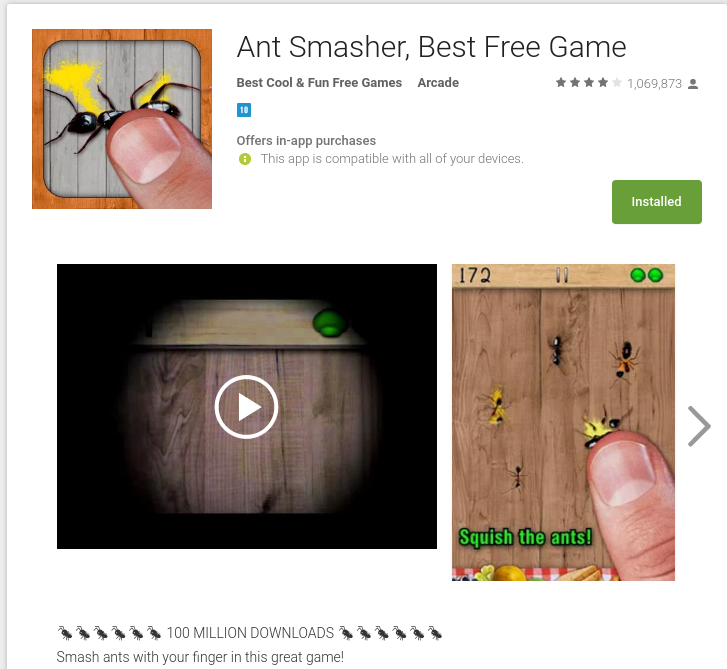
\includegraphics[scale=0.5]{img/antsmasherGooglePlay}}
\label{fig:antsmasherGooglePlay}
\caption* {Fonte: https://play.google.com/store/apps/details?id=com.bestcoolfungames.antsmasher}
\end{figure}

Grande parte do fluxo de receita da BCFG vinha através de publicidade em seus jogos. Como mostra a \autoref{fig:antsmasheriOS}
\begin{figure}[H]
\caption{Banner de propaganda no Ant Smasher para iOS}
\centerline{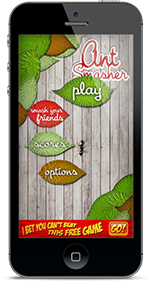
\includegraphics[scale=0.5]{img/antsmasheriOS}}
\label{fig:antsmasheriOS}
\caption* {Fonte: Website Revmob - https://www.revmobmobileadnetwork.com/site}
\end{figure}

Na época haviam poucas redes de propaganda que proviam um serviço de baixa qualidade para os desenvolvedores de aplicativos. Sabiamente, o fundador da BCFG resolveu criar sua própria rede de propagandas, para tirar proveito desse mercado. Surgiu então em 2011 a Revmob (RM), que rapidamente se tornou a maior rede de propagandas para aparelhos móveis da América Latina, mesmo não tendo focado tanto no mercado brasileiro. Em 2015 a empresa buscou dar mais atenção ao Brasil buscando mais anunciantes e desenvolvedores de aplicativos brasileiros. Para alinhar com essa estratégia fez uma versão em português do \textit{website} da empresa como mostra a \autoref{fig:screenshotSiteRev}.

\begin{figure}[H]
\caption{Website RevMob para o Brasil}
\centerline{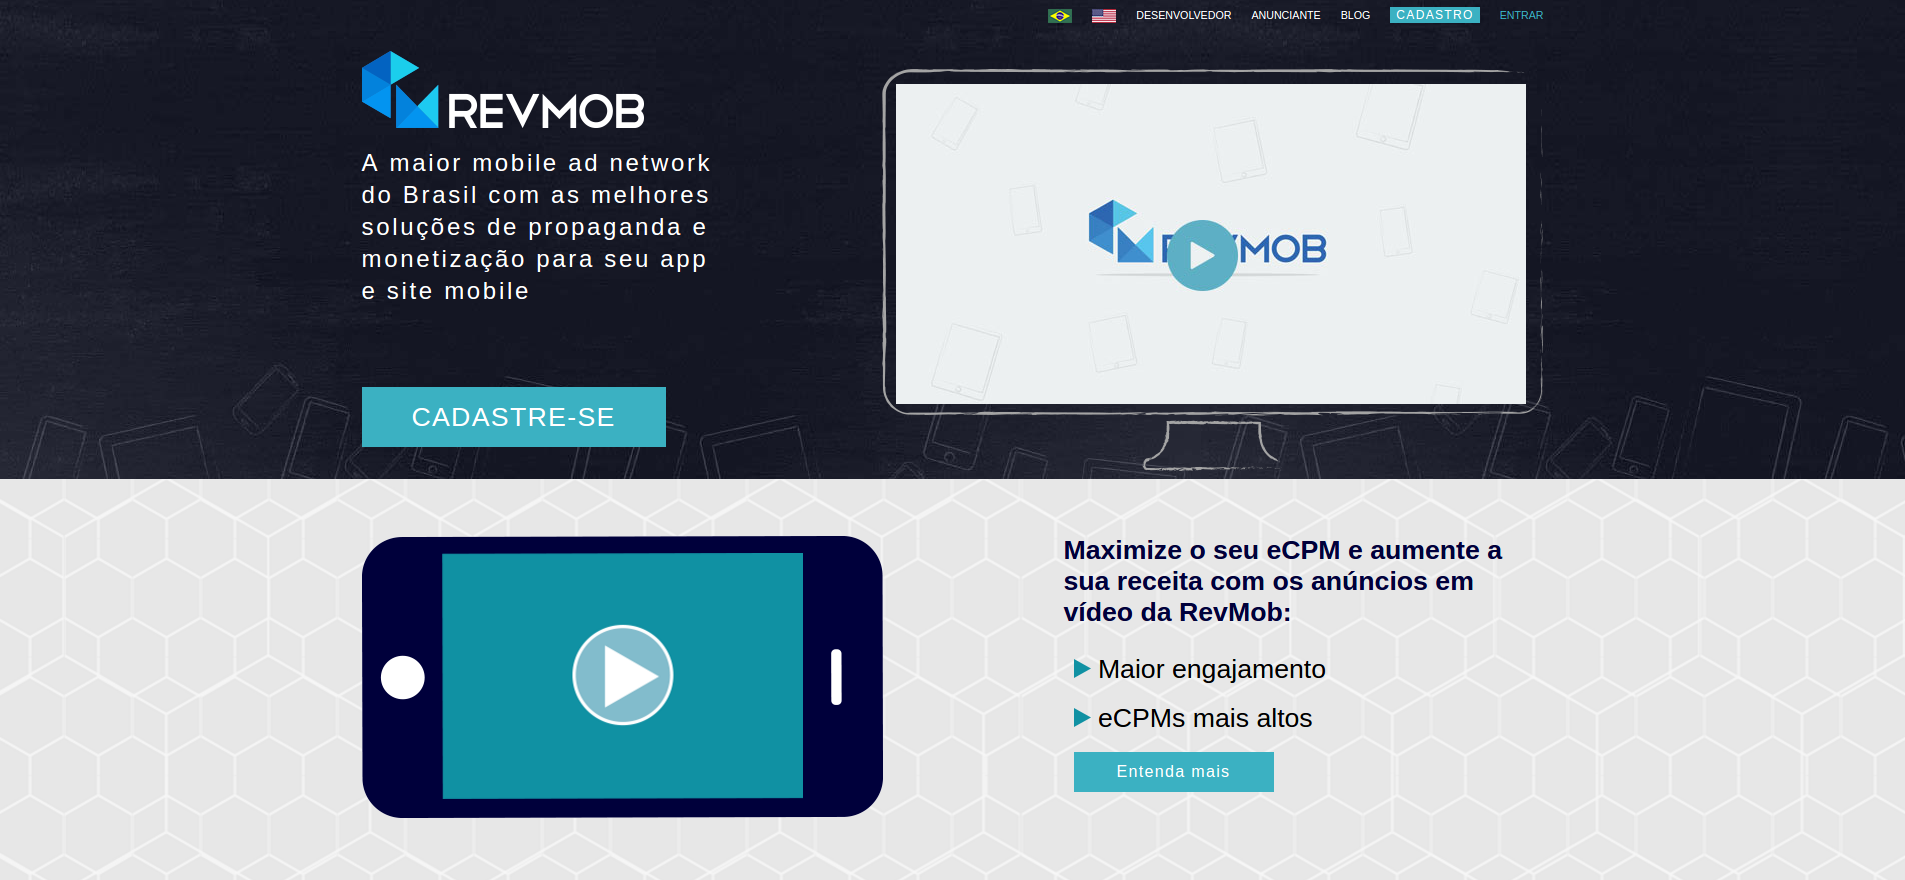
\includegraphics[width=0.8\textwidth]{img/screenshotSiteRev}}
\label{fig:screenshotSiteRev}
\caption* {Fonte: Website Revmob - https://www.revmobmobileadnetwork.com/site}
\end{figure}

O mercado de redes de anúncio cresceu rapidamente e se tornou muito competitivo. As grandes vantagens competitivas nesse mercado são:
\begin{itemize}
\item Servir rapidamente o anúncio, baixa latência, em questão de menos de 100 milissegundos.
\item Saber estimar as taxas de conversão de um anúncio. Para cada vez que o anúncio aparecer qual a chance dele ser clicado, e para cada clique qual a chance do aplicativo ser instalado.
\item Saber aumentar as taxas de conversão de uma propaganda. Geolocalização precisa e saber as informações da pessoa para o qual o anúncio está sendo mostrado aumentam bastante as taxas de conversão.
\end{itemize}

O desafio da latência foi resolvido através de uma reestruturação dos sistemas e de reescrita do código. Para endereçar o desafio da estimativa das taxas de conversão foi necessária a criação de uma nova empresa chamada Beluga, criada em 2014. As soluções de Big Data eram demasiadamente caras e de difícil integração com o sistema da Revmob. E sobre o aumento das taxas de conversão a Revmob decidiu focar na questão da geolocalização precisa, através da tecnologia de beacons, o que culminou no nascimento da empresa Beeconnect em 2015, que será o foco desse trabalho de formatura.

\section{Contexto da Beeconnect}
\label{cha:contexto_da_beeconnect}
A Beeconnect surgiu para externalizar os conhecimentos obtidos com as demais empresas do grupo Techmob. A empresa nasceu com 4 pessoas com a supervisão de um membro do Board da Techmob.

A empresa queria tirar proveito da tecnologia de beacons que estava na moda em 2015, porém poucos no Brasil tinham ouvido falar, o que poderia ser uma vantagem competitiva. O beacon é um aparelho que utiliza a tecnologia \textit{Bluetooth Low Energy} ou BLE que pode ser utilizado para geolocalização interna com uma ótima precisão, superando em muito o GPS para locais internos como Shoppings, por exemplo.

A equipe fez diversas análises de como os beacons estavam sendo utilizados no exterior e descobriu diversas aplicações em lugares diversos como shoppings, vide \autoref{fig:beaconShopping}, aeroportos, hospitais, hotéis e museus. O time estava ansioso para testar essa tecnologia em alguma aplicação mas ainda não tinha ideia do que fazer.

\begin{figure}[H]
\caption{Aplicação de beacon em shopping}
\centerline{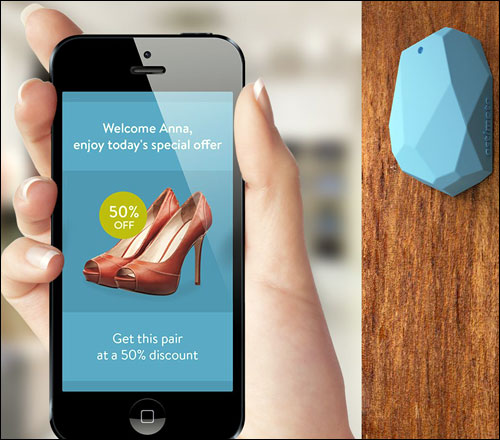
\includegraphics[scale=0.5]{img/beaconShopping}}
\label{fig:beaconShopping}
\caption* {Fonte: Material de marketing da Estimote - fornecedora de beacons}
\end{figure}

Até que um dos membros da equipe utilizou um contato que trabalhava em um grande shopping da capital paulista e agendou uma reunião para apresentar a tecnologia de beacons e o valor que a Beeconnect conseguiria gerar para eles. Dado o histórico da Techmob com propagandas em dispositivos móveis o time acabou optando por criar um aplicativo que disparava uma notificação assim que o celular entrasse em um raio de meio metro do beacon. Rapidamente a equipe desenvolveu  um produto que serviria para mandar propagandas geolocalizadas, trabalhando cerca de 16 horas por dia por uma semana, que consistia em:
\begin{itemize}
\item Um aplicativo para iOS que possuía um SDK (basicamente um software) que permitia a comunicação com beacons.
\item Um servidor que fazia a comunicação com o aplicativo e gravava todas as informações de distância do celular em relação ao beacon e enviava uma propaganda para o aplicativo.
\end{itemize}

Porém na apresentação para o Shopping a equipe sequer apresentou o produto desenvolvido dado o desenrolar dado que o cliente claramente não parecia interessado com a ideia de publicidade móvel feita de dessa maneira.

Todos ficaram muito frustrados com o tempo perdido e a sensação de que haveria um jeito melhor de ter desenvolvido o projeto sem ter gasto esforços com tarefas desnecessárias ou que não tinham um valor claro a ser gerado.

A equipe então começou a vender a ideia do que a Beeconnect poderia fazer e criar o produto junto com o cliente. Basicamente utilizou-se o processo de vender apresentações em slides para validar a ideia de que uma ferramenta de geolocalização precisa tem valor. Foram feitas reuniões com diversos tipos de clientes: hospitais, hotéis, construtoras, concessionárias e varejistas. Após essas reuniões o foco da empresa ficou mais claro. O varejo pareceu ser a opção mais rentável pois trata-se de um mercado gigantesco e que tem uma necessidade de saber mais sobre os consumidores.

Após acumular alguns varejistas interessados ficou evidente a necessidade da criação de um produto para ser testado. A pressão por resultados fez até o autor abrir mão da graduação na Escola Politécnica para trabalhar cerca de 14 horas por dia para liderar o desenvolvimento tanto de um servidor quanto de um aplicativo para smartphones \textit{Android}. Dado o aparente interesse dos varejistas por essa tecnologia a Beeconnect realizou mais contratações para auxiliar tanto em vendas quanto no desenvolvimento de software.

O produto criado foi um aplicativo de descontos chamado iShop, que utilizava a tecnologia de beacons para gerar um cupom de desconto somente na loja física cadastrada. O funcionamento do aplicativo basicamente consistia em quatro etapas conforme mostrado na \autoref{fig:explicacaoBeeconnect}:
\begin{itemize}
\item Comunicação do celular com o beacon: O beacon é um aparelho passivo, ou seja, ele só emite um sinal mandando três informações: \textit{UUID}, \textit{Major} e \textit{Minor}. O \textit{UUID} é o identificador único universal, trata-se de um número hexadecimal de trinta e dois dígitos que para o caso dos beacons tem como propósito identificar uma rede de beacons. Já o \textit{Major} e \textit{Minor} são números inteiros que variam de 0 a 65535 que têm como objetivo identificar um beacon dentro da rede dele.
\item Interação do usuário com o aplicativo: com o aplicativo o usuário consegue ver as ofertas mais relevantes para ele, consultar as lojas mais próximas a ele e gerar cupons de desconto.
\item Comunicação do celular com o servidor: O aplicativo só funciona se o usuário estiver conectado a internet, seja por meio do 3G/4G ou via \textit{WiFi}. O servidor então manda para o celular as ofertas mais relevantes baseadas na localização do usuário enviada pelo celular. Além disso, o celular envia para o servidor qual beacon que ele está detectando para que o servidor decida ou não enviar uma notificação para o usuário.
\item Interação do varejista com a plataforma: Para o varejista foi criada uma plataforma, um site, onde ele consegue gerenciar as informações e as promoções de cada loja. Tais dados são então salvos na base de dados e então disponibilizados para o aplicativo.
\end{itemize}

\begin{figure}[H]
\caption{Funcionamento app Beeconnect}
\centerline{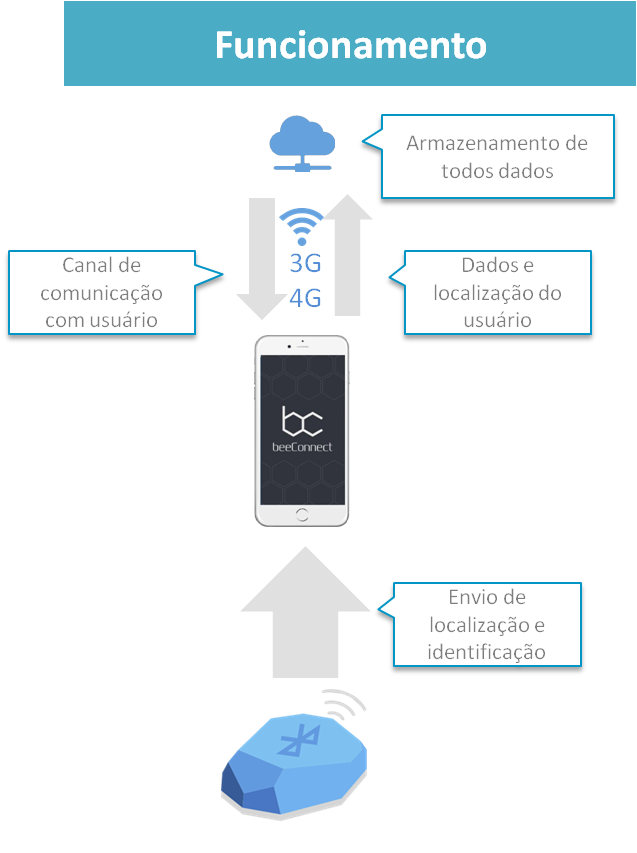
\includegraphics[scale=0.75]{img/explicacaoBeeconnect}}
\label{fig:explicacaoBeeconnect}
\caption* {Fonte: Material de marketing da Beeconnect}
\end{figure}

O primeiro piloto para testar esse produto foi realizado no McDonald's localizado na Riviera de São Lourenço. Foram disponbilizadas cinco ofertas para o aplicativo, desde McOfertas até sobremesas e bebidas.
Houve a geração e utilização de alguns cupons no local, entretanto nada muito relevante. Todos os usuários que baixaram o aplicativo acharam muito simples e fácil de gerar o desconto, entretanto poucas pessoas o baixaram. A distância entre o local do piloto e o escritório da Techmob deixava inviável um acompanhamento de perto. 

Além disso, por motivos estratégicos a matriz do McDonald's do Brasil pediu para que o piloto fosse cancelado. E no meio de toda essa turbulência, o advogado da Techmob sugeriu que o nome do aplicativo fosse mudado porque dificilmente algum nome de marca com "i" como prefixo seria registrado, pois já é praticamente um consenso que esse prefixo remete aos produtos e serviços da marca \textit{Apple}. Assim, a equipe decidiu registrar a marca Beeconnect e utilizá-la como nome do aplicativo também. Foi necessária também uma reformulação no design do aplicativo para que ficasse condizente com a marca.

Após tais insucessos e com muito esforço a empresa conseguiu fechar um piloto com o maior varejista da América Latina, o Grupo Pão de Açúcar. Foi realizado um piloto na loja dentro da sede da empresa. A promoção foi "Todas as cervejas premium com 50\% de desconto". O resultado foi um sucesso. Vários funcionários baixaram o aplicativo na hora e conseguiram utilizar o desconto sem problemas. O resultado do piloto foi um contrato assinado no qual seriam implementados beacons em todas as lojas de formato de proximidade premium, chamadas de Minuto Pão de Açúcar, no estado de São Paulo.

Após a implementação dos beacons em todas as Minuto Pão de Açúcar, esperou-se um resultado condizente com o esforço. Infelizmente tal resultado não veio. A pressão resultados do board da Techmob veio. A holding havia gasto cerca de R\$500.000 reais até então.

\section{Definição do problema}
\label{cha:definição_do_problema}
A Beeconnect estava prestes a ser um projeto engavetado. A empresa já gastara cerca de meio milhão de reais no decorrer de um ano, entre os seus principais custos envolvem os recursos humanos. Dado que o time dessa startup era muito bem qualificado, praticamente todos os integrantes do time eram engenheiros formados ou estudantes de engenharia pela Escola Politécnica, e que havia outras frentes da Techmob que também necessitavam de recursos o Conselho da holding começou a pressionar a Beeconnect para gerar resultados, caso contrário, eles iriam começar a desmontar o time para suprirem outras áreas da holding.

O principal problema é que a startup ainda não sabia se possuía um modelo de negócio sustentável e que gera valor para seus clientes. A empresa encontrava-se em momento no qual tinha um grande primeiro cliente, que entretanto estava em modo de testes, ou seja, não estava pagando.
Todo o negócio da empresa começou sem ter um planejamento ou alguma base teórica para fomentar um desenvolvimento mais sólido do negócio. Tudo isso foi agravado pelo fato da empresa ter crescido em número de funcionários sem ter provado o modelo de negócio, o que acabou inflando os custos.

A empresa sequer tinha feito um Canvas de Modelo de Negócio para que todos da equipe conseguissem ter uma visão geral do projeto e poderem opinar e iterar em cima do modelo. Dessa forma pelo fato da Beeconnect ter começado mal estruturada, praticamente um ano havia se passado e ainda não estava claro se a empresa deveria perseverar em seu modelo de negócio, pivotar para outro tipo de negócio ou simplesmente fechar a empresa e realocar os recursos para outras áreas.

Além disso, faltavam mais lojas para validar a proposta de valor da Beeconnect no lado dos varejistas assim como faltavam mais usuários para verificar se eles enxergavam valor no aplicativo. A Beeconnect encontrava-se no clásssico problema do "Ovo e da Galinha", no qual os varejistas reclamavam que a base de usuários do aplicativo era muito pequena e só entrariam quando a base fosse maior. No caso dos usuários muitos faziam reclamações sobre o baixo número de lojas que os interessavam.

\section[Objetivos]{Objetivos}
\label{chap:objetivos}
Dado o problema apresentado fica evidente que a Beeconnect precisa ser estruturada de modo a virar uma máquina de testar hipóteses para que a startup itere o mais rápido possível de forma a encontrar o seu modelo de negócio.
A reestruturação deve visar responder se a Beeconnect gera valor para seus clientes, tanto para os varejistas quanto para os usuários do aplicativo. O modelo a ser seguido deverá seguir a literatura ligada ao empreendedorismo, principalmente a de \citeonline{leanstartup}, \citeonline{businessmodel} e \citeonline{startupowners}

\section{Justificativa}
\label{cha:justificativa}
Para o autor a importância do tema desse trabalho é imensa dado que a Beeconnect tem sido basicamente a vida dele durante o último ano. Foram madrugadas trabalhando, noites mal dormidas, finais de semana perdidos, graduação postergada para que a Beeconnect saísse do papel e conquistasse o varejo físico brasileiro, talvez mundial.

Para a Techmob verifica-se a relevância de utilizar os métodos propostos pela literatura e como isso pode fazer diferença na hora de começar novas empresas bem como tal iniciativa pode trazer economias para testar novas hipóteses.

Dado que o espírito empreendedor está cada vez mais forte dentro da Escola Politécnica da Universidade de São Paulo. O trabalho aqui apresentado mostra a relevância do ensino de tais métodos de empreendedorismo, para que as futuras startups criadas por politécnicos não tenham um início tão turbulento quanto a empresa analisada neste trabalho. E caso a startup também saia mal estruturada assim como a Beeconnect que esse trabalho de conclusão de curso seja um material de referência para auxiliar empresas que estão passando por um processo de reestruturação.

Para a sociedade a importância é mostrar que no empreendedorismo não basta ter uma boa ideia, parece que todo mundo quer fazer um aplicativo. É necessário que essa ideia seja bem estruturada e o mais importante, que ela seja validada o mais rápido possível. É importante apresentar que o mundo empreendedor não é glamuroso como se mostram nos filmes e nas revistas, que não é nada fácil construir o próximo \textit{Facebook} ou \textit{Google}. É preciso demonstrar que a escolha de empreender tem que vir com a vontade de passar por dificuldades, por momentos de estresse. O empreendedor tem que ser resiliente. 

%\input{requisitos}
%!TEX root = index.tex
\chapter{Testes e Resultados}
\label{cha:testes_e_resultados}
Conforme apresentado anteriormente, o produto da empresa Beeconnect é o aplicativo com o mesmo o nome. Tal produto foi desenvolvido para as plataformas Android e iOS e consiste basicamente em um aplicativo para descontos em lojas físicas. O seu principal diferencial é a geolocalização indoor precisa com uso de um aparelho chamado beacon. Quando um usuário do aplicativo passar por um beacon localizado dentro de uma loja parceira ele pode receber uma notificação informando que ele recebeu um desconto especial em um produto relevante ou receber um simples "Bem vindo" conforme mostrado na \autoref{fig:bemvindo_beeconnect}.

\begin{figure}[H]
\caption{Exemplo de notificação do aplicativo Beeconnect}
\centerline{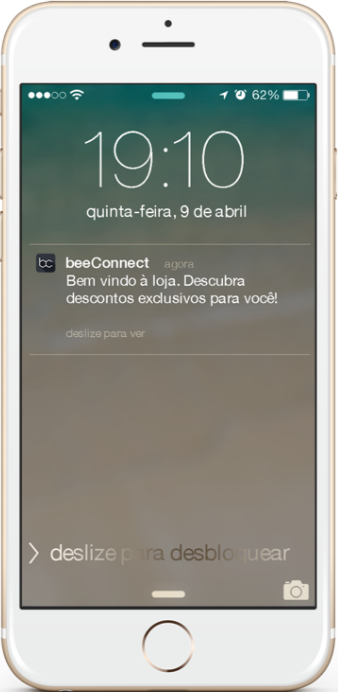
\includegraphics[scale=0.35]{img/bemvindo_beeconnect}}
\label{fig:bemvindo_beeconnect}
\caption* {Fonte: https://app.beeconnect.com.br/}
\end{figure}

Até o momento em que os testes foram realizados a Beeconnect contava com cerca de 2000 downloads do aplicativo, 1600 usuários cadastrados e 10 empresas parceiras. Um dos problemas é que nenhuma loja ainda estava disposta a pagar pela plataforma.

Os principais desafios da Beeconnect são:
\begin{itemize}
\item Crescer a base de lojas pagantes do aplicativo.
\item Crescer a base de usuários de forma barata.
\end{itemize}

Como mencionado previamente tais desafios eram realmente difíceis de serem resolvidos porque muitos usuários só baixariam o aplicativo se ele possuísse mais lojas participantes, assim como muitas lojas só se interessavam pela base de usuários e só entrariam no aplicativo caso a base fosse grande, com mais de cem mil usuários.

Baseando-se na metodologia apresentada no capítulo anterior o autor então começou a desenvolver os testes e resultados que serão apresentados nesse capítulo. Foram feitas duas iterações no ciclo explicitado pela metodologia introduzida no capítulo anteriror.

\section{Mapear estado atual da startup}
\label{cha:mapear_estado}
O autor elaborou um canvas inicial, ilustrado na \autoref{fig:canvas_beeconnect_1}, baseado nas premissas iniciais da empresa: 

\begin{figure}[H]
\caption{Canvas de Modelo de Negócio inicial da Beeconnect}
\centerline{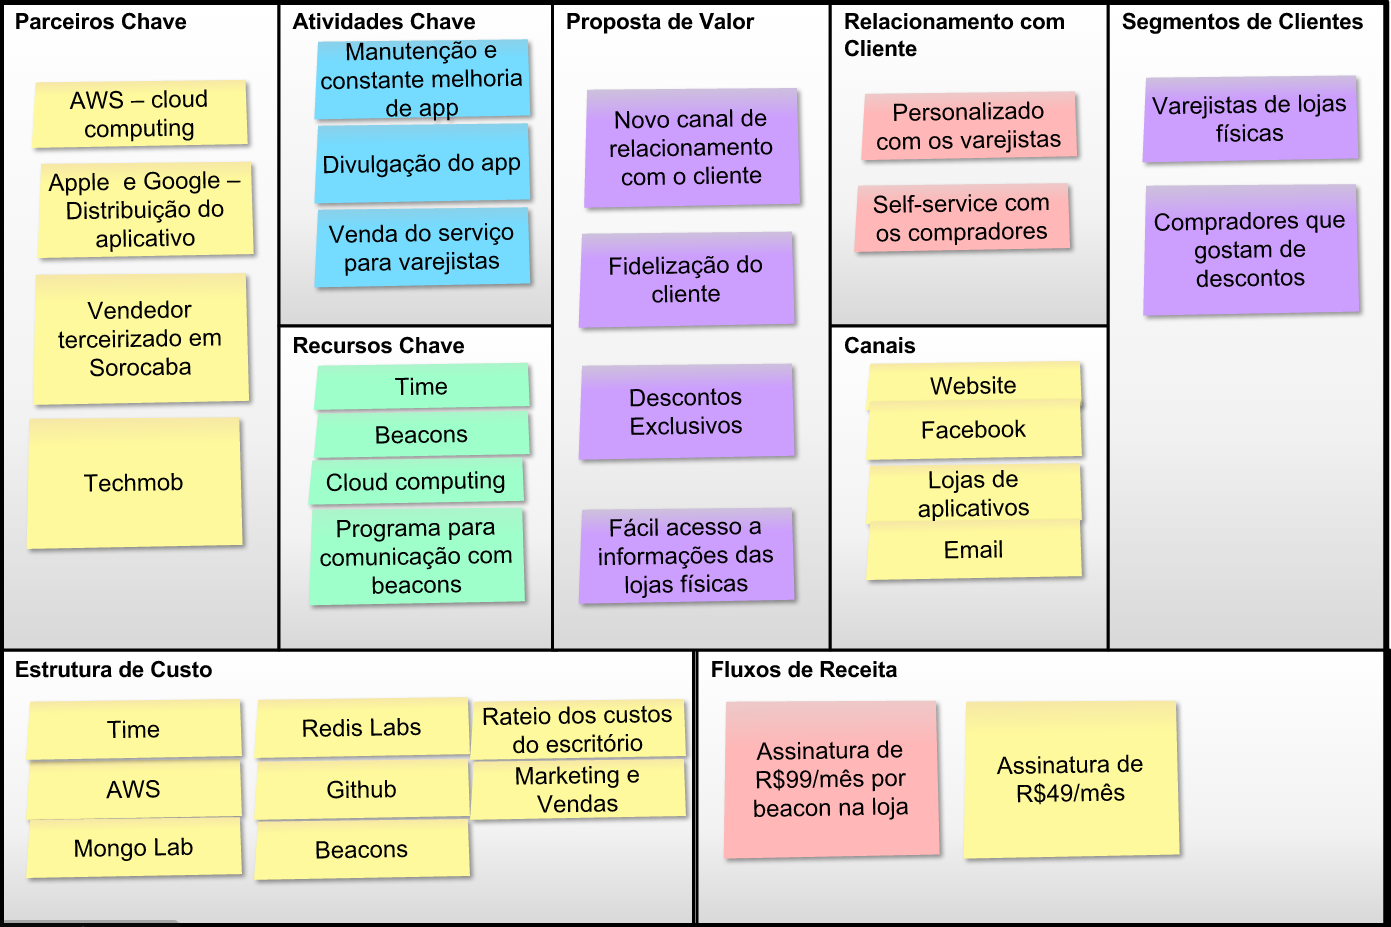
\includegraphics[scale=0.25]{img/canvas_beeconnect_1}}
\label{fig:canvas_beeconnect_1}
\caption* {Fonte: Elaborado pelo autor}
\end{figure}

Foram detalhados então cada um dos nove blocos do Canvas de Modelo de Negócio.
\subsection{Segmentos de Clientes}
\label{cha:segmentos_de_clientes}
Os segmentos de clientes para o aplicativo são:
\begin{itemize}
\item Varejistas de lojas físicas, que serão tratados daqui em diante como "Lojas": 
\item Frequentadores de lojas físicas que gostam de descontos, que serão tratados aqui em diante como "Usuários": 
\end{itemize}
Deste modo verificou-se que o produto atende dois segmentos distintos porém dependentes, típico de um mercado Multilateral. Por exemplo: sem uma boa diversidade de Lojas participantes no aplicativo não há muitas opções de descontos para os Usuários.

\subsection{Proposição de Valor}
\label{cha:proposicao_de_valor}
Dado que o produto atende um segmento multilateral de clientes ele tem que gerar valor para ambos os segmentos.
\begin{itemize}
\item Novo canal de relacionamento com o cliente: os lojas físicas tem no aplicativo uma nova plataforma para se comunicar com seus clientes. Elas podem enviar notificações para eles quando ele passar em um raio de quinhentos metros de uma de suas lojas, graças a tecnologia do GPS. Além disso, o cliente pode consultar as promoções de uma determinada loja sem precisar sair de casa.
\item Fidelização do cliente: graças a tecnologia de beacon o lojista consegue saber quantas vezes cada cliente foi a sua loja a premiá-lo de acordo com isso seja com descontos ou com algum brinde.
\item Descontos Exclusivos: é a principal proposta de valor para os Usuários. Mais uma vez graças a tecnologia de beacons o aplicativo consegue saber quando que o usuário está próximo de um determinado produto e oferecer um desconto exclusivo.
\item Fácil acesso a informações das lojas físicas: o usuário pode facilmente consultar onde fica a loja de supermercado mais próxima a ele, ver seu endereço e já rapidamente colocar no endereço no GPS.
\end{itemize}

\subsection{Relacionamento com Cliente}
\label{cha:relacionamento_com_cliente}
Dado que as Lojas serão os clientes pagantes e o número é bem menor que o de usuários do aplicativo a empresa optou por oferecer uma comunicação personalizada com os varejistas e uma comunicação automatizada com os usuários. 

\subsection{Canais}
\label{cha:canais}
Os principais canais são:
\begin{itemize}
\item Website: com o \textit{site} https://app.beeconnect.com.br/ é possível atender tanto o usuário quanto o lojista. Nele o lojista pode fazer fazer o gerenciamento das campanhas que irão aparecer no aplicativo. Já o usuário pode saber mais sobre o aplicativo.
\item Facebook: a página do aplicativo no Facebook, https://www.facebook.com/beeconnectbr/, foi feita com o intuito de conseguir fazer campanhas para conseguir mais usuários para o aplicativo, mas também é um canal de interação com as Lojas dado que é possível, por exemplo, mencionar a loja em um publicação da página da Beeconnect.
\item Relações Públicas: dado que a BC faz parte do grupo TM que possui uma assessoria de relações públicas há chances da BC aparecer em reportagens.
\item Lojas de Aplicativos: as lojas de aplicativos \textit{App Store} do sistema operacional iOS e \textit{Play Store} do sistema operacional Android são de extrema importância pois são nelas que o usuário consegue baixar o aplicativo para o celular. 
\item Email: Através do email marketing é possível se relacionar com os usuários já existentes para informá-los sobre novas lojas parceiras ou sobre descontos super especiais.
\end{itemize}

\subsection{Fluxos de Receita}
\label{cha:fluxos_de_receita_canvas_bc_1}
A empresa optou por oferecer dois métodos de cobrança dos lojistas:
\begin{itemize}
\item Assinatura de R\$99 por mês por beacon por loja: assim se uma loja optar por utilizar 2 beacons ela terá que pagar R\$198 por mês. Nessa assinatura o lojista ganha acesso a todas as opções como enviar uma notificação assim que o cliente entra na loja, acesso ao número de visitantes que passaram pela loja, entre outras funcionalidades.
\item Assinatura de R\$49 por mês por loja: a empresa optou por oferecer essa modalidade de assinatura para o caso do lojista não ver valor no uso dos beacons. Assim ele só conta com a funcionalidade de enviar notificações para os usuários estiverem a um raio de quinhentos metros de sua loja e disponibilizar seus produtos na vitrine virtual do aplicativo.
\end{itemize}

\subsection{Parcerias Chave}
\label{cha:parcerias_chave}
As parcerias-chave da Beeconnect são:
\begin{itemize}
\item Amazon Web Services: A Amazon Web Services, popularmente conhecida como AWS é o serviço de computação em nuvem da Amazon, maior site de compras \textit{online} dos Estados Unidos. A AWS é de fundamental importância para um negócio que envolve servidores, gracas a ela muitos negócios se tornam viáveis por é possível testar hipóteses sem gastar muito dinheiro para construir toda uma infraestrutura de servidores por trás. Com a AWS o empreendedor só paga por hora de máquina utilizada e dá para facilmente colocar uma máquina melhor caso a infraestrutura necessite para suportar um tráfego maior.
\item Apple e Google: Um desenvolvedor de aplicativos pode se manter fora das lojas de aplicativos da Apple e do Google, entretanto se ele quiser ser levado a sério ele tem que passar por todo o trâmite de aprovação de seu aplicativo para poder disponibilizá-lo nas lojas oficiais. 
\item Vendedor terceirizado: Um vendedor entrou em contato com a equipe pois ele acabou sabendo do produto e achou interessante. Ele acabou propondo vender o produto mediante a uma comissão de 20\% por venda. Dado que o time de vendas da BC é bem enxuto a equipe achou interessante a proposta dado que só haveria um custo variável por venda realizada.
\item TM: Poucas empresas tem a chance de serem criadas dentro de um grupo que já possui startups lucrativas. A TM forneceu uma estrutura muito boa para o desenvolvimento da Beeconnect.
\end{itemize}

\subsection{Atividades Chave}
\label{cha:parcerias_chave}
As atividades Chave da Beeconnect são:
\begin{itemize}
\item Manutenção e constante melhoria do aplicativo: os desenvolvedores devem sempre estar atentos à mudanças nos sistemas operacionais. Por exemplo: em 2015 com o lançamento da versão 9 do sistema da Apple alguns códigos tiveram que ser alterados caso contrário o aplicativo não iria funcionar, o mesmo aconteceu para a versão \textit{Marshmallow} do sistema operacional da Google. Além disso, os desenvolvedores necessitam colocar mais funcionalidade ao aplicativo além de possibilitar a realização de testes A/B na interface para que ela seja a mais intuitiva possível.
\item Divulgação do Aplicativo: O desafio conforme explicado por \citeonline{mcclure2007startup} é conseguir o meio mais barato de adquirir bastantes usuários. O custo de aquisição de usuários deve ser menor que a receita gerada por cada usuário.
\item Venda do serviço para varejistas: Assim como a base de usuários tem que crescer, a base de lojas também deve crescer junto. Por se tratar de um negócio multilateral quanto mais lojas melhor para os usuários, assim como quanto mais usuários melhor é para as lojas.
\end{itemize}

\subsection{Recursos Chave}
\label{cha:recursos_chave}
Os Recursos Chave da Beeconnect são:
\begin{itemize}
\item Time: A equipe é bem qualificada, praticamente toda formada por engenheiros e estudantes de engenharia da Escola Politécnica da USP.
\item Beacons: Os beacons são equipamentos pouco conhecidos no mercado brasileiro, entretanto, já estão sendo utilizados amplamente nos Estados Unidos. Esses aparelhos são relativamente baratos se comparados com outras ferramentas de localização interna. 
\item Computação em nuvem: Conforme citado anteriormente a computação em nuvem permite que a empresa possa testar suas hipóteses e criar seus negócios sem que haja um investimento adiantado em servidores. Nesses servidores ficam os códigos responsáveis pela comunicação com o aplicativo e pela interação do usuário com o site da Beeconnect.
\item Programa para comunicação com beacons: Os desenvolvedores tiveram que fazer um programa que possibilita a comunicação com beacons. Tal \textit{software} possibilita a comunicação entre o celular do usuário com o beacon, além disso, ele já envia para os servidores da Beeconnect qual beacon que o celular está captando, assim o servidor pode mandar uma promoção especial para o usuário que está naquela loja. Esse \textit{software} pode ser instalado em outras aplicações que queiram se comunicar com os beacons da Beeconnect.
\end{itemize}

\subsection{Estrutura de Custo}
\label{cha:estrutura_de_custo}
A Estrutura de Custo da Beeconnect é descrita abaixo:
\begin{itemize}
\item Time: A equipe é responsável pela maior parte dos custos da empresa. Com cerca de 12 membros no time, a Beeconnect gasta quase R\$100.000 em recursos humanos.
\item Rateio do aluguel e despesas do escritório: A TM possui um escritório localizado na Rua Haddock Lobo. O aluguel e demais despesas do escritório são rateados proporcionalmente ao número de integrantes por empresa da TM.
\item Beacons: Os aparelhos são importados da China. Cada aparelho sai por cerca de R\$100 já com impostos e frete.
\item Marketing e Vendas: Nesse item podem ser considerados as custos das campanhas de marketing digital e físico bem como os gastos para visitar clientes.
\item Mongo Lab: É o serviço de base de dados utilizado para guardar os dados dos usuários, campanhas, lojas. Gasta-se cerca de R\$600 por mês com esse serviço para armazenar até 40 Gb
\item Redis Labs: É um outro serviço de base de dados, esse tipo de base é muito mais rápido pois ele um tipo de memória de acesso mais rápido, entretanto o custo de armazenamento é mais caro. Gasta-se cerca de R\$60 por mês para o armazenamento de até 0.5 Gb
\item Github: é um serviço de armazenamento, versionamento e compartilhamento de código.
\item AWS: Como dito anteriormente, é o serviço de computação em nuvem da Amazon. A Beeconnect utiliza cerca de 20 máquinas e gasta por volta de R\$1600 por mês.
\end{itemize}

\section{Gerar hipóteses sobre a proposta de valor da empresa}
\label{cha:gerar_hipoteses}
Dada a situação inicial da empresa modelada no Canvas de Modelo de Negócio e o objetivo do trabalho de formatura de provar que a Beeconnect tem um modelo de negócio sustentável, o autor recorreu a literatura para buscar a melhor alternativa de solução para o problema. 
Segundo a literatura o principal problema de uma startup é construir um produto que ninguém quer. Em outras palavras, o maior problema é o produto construído ou serviço prestado não gerar valor para seu cliente.
Ficou evidente que era urgente verificar se o aplicativo gerava valor para seus usuários. Baseando-se nas métricas pirata de \citeonline{mcclure2007startup}, na análise de coorte de \citeonline{leanstartup} e no Canvas de Modelo de Negócio, nos itens Segmentos de Clientes e Proposição da Valor, foram elaboradas as seguintes hipóteses:
\begin{itemize}
\item Hipótese 1: \textbf{Varejistas de lojas físicas tem interesse num novo canal de relacionamento com os clientes}. O objetivo era verificar se os varejistas estavam interessados em se comunicar com seus clientes através de notificações em \textit{smartphone} além dos canais tradicionais como email, telefone, panfletos entre outros.
\item Hipótese 2: \textbf{Varejistas de lojas físicas tem interesse em fidelizar o cliente}. O objetivo era testar se os varejistas estavam dispostos a dar algum benefício aos seus clientes antigos para que eles voltassem cada vez mais às suas lojas.
\item Hipótese 3: \textbf{Post no \textit{Facebook} focando os simpatizantes de uma determinada marca é um meio barato e efetivo de adquirir clientes}. O teste de tal hipótese visava verificar se o \textit{Facebook} seria um bom meio de conseguir novos usuários para o aplicativo dado que o crescimento rápido da base de usuários de um modo barato era de extrema importância para o sucesso do negócio. Já se sabia de antemão que o marketing nessa rede social era um pouco caro, entretanto, a dúvida que restava era se o foco em determinado público ajudaria a aumentar a conversão de modo a reduzir o custo um novo usuário.
\item Hipótese 4: \textbf{É fácil de gerar cupons na primeira semana de uso do aplicativo}. Tal hipótese visava testar a questão da Ativação do usuário apontada por \citeonline{mcclure2007startup}. Infelizmente, devido a falta de integração com os sistemas de vendas dos varejistas era impossível a verificação automática se o usuário havia de fato \textbf{utilizado} do cupom de desconto. Portanto, para a equipe da Beeconnect o usuário só era considerado ativo se ele tivesse \textbf{gerado} pelo menos um cupom. 
\item Hipótese 5: \textbf{Os usuários que geraram cupom utilizam o aplicativo na segunda semana}. O intuito de verificar essa hipótese baseia-se no conceito de Retenção do usuário mencionado tanto por \citeonline{mcclure2007startup} como por \citeonline{leanstartup}. O usuário só seria considerado retido se ele estivesse gerando cupons constantemente no aplicativo.
\item Hipótese 6: \textbf{Clientes que gostam de desconto tem interesse em fácil acesso às informações das lojas físicas}. Dado o contexto que os usuários do aplicativo são frequentadores de lojas físicas a equipe da Beeconnect achou que seria útil construir uma página com informações sobre a loja como localização com integração com o sistema do \textit{Google Maps} e inclusive com um que levava ao GPS do \textit{smartphone}. Tais funcionalidades foram uma das que mais demandaram tempo do time de desenvolvimento sendo que não houve nenhuma demanda clara por parte dos usuários. O objetivo seria testar se os usuários realmente utilizariam essa funcionalidade ou se ela foi feita em vão. 
\end{itemize}

\section{Desenhar Testes de Hipóteses}
\label{cha:desenhar_hipoteses}
Uma vez que as hipóteses foram elaboradas foi necessário estruturar a maneira como tais hipóteses seriam testadas. 

\subsection{Hipótese 1}
\label{cha:hip_1}
Para a hipótese "Varejistas de lojas físicas tem interesse num novo canal de relacionamento com os clientes" o teste proposto foi organizar um mutirão de vendas e sair para a rua, na região dos Jardins devido a proximidade com o escritório da Beeconnect e tentar vender o serviço. A métrica de sucesso definida foi:
\[ \dfrac{NLP}{LV} > 10\%\]

Onde: 
\begin{itemize}
\item NLP: é o número de novas lojas parceiras que foram adquiridas durante o mutirão de vendas.
\item LV: é o número de lojas visitadas durante o mutirão de vendas.
\end{itemize}

\subsection{Hipótese 2}
\label{cha:hip_2}
Para a hipótese "Varejistas de lojas físicas tem interesse em fidelizar o cliente" os vendedores da Beeconnect deveriam ligar para os varejistas que já estavam participando no aplicativo e propor que eles oferecessem pelo um produto com desconto exclusivo para o aplicativo de formar a fidelizar os clientes. Nesse caso a métrica de sucesso definida foi:

\[\dfrac{LCD}{LP} > 40\%\]

Onde: 
\begin{itemize}
\item LCD: é o número de lojas que disponibilizaram pelo menos um cupom de desconto exclusivo.
\item LP: é o número de lojas participantes no aplicativo, ou seja, lojas que já estavam com pelo menos alguma campanha disponível no app.
\end{itemize}

Para as demais hipóteses o teste proposto foi analisar um certo grupo de usuários e verificar como eles se comportariam com o passar do tempo. 

\subsection{Hipótese 3}
\label{cha:hip_3}
O primeiro passo consistiria na criação de um anúncio pago no Facebook colocando como alvo as pessoas que deram "curtir" na página em um dos parceiros do aplicativo na época. A métrica utilizada para testar a hipótese "Post no Facebook para simpatizantes da marca é um meio barato e efetivo de adquirir clientes" foi:
\begin{align*} 
CAC < R\$1,00 \\
\dfrac{D}{AP} > 0.5\%
\end{align*}

Onde: 
\begin{itemize}
\item CAC: é o custo de aquisição de um usuário. É o custo de marketing para conseguir um novo usuário do aplicativo. Um dos grandes objetivos das startups é ter um CAC menor que o valor do ciclo de vida do cliente que basicamente é todo o valor gerado pelo cliente durante o uso do aplicativo.
\item D: é o número de downloads do aplicativo advindos do post no \textit{Facebook}.
\item AP: é o alcance da publicação, ou seja, quantas pessoas diferentes viram a publicação feita no Facebook. O grande desafio é fazer com que as pessoas interajam com a publicação paga, pois a cada comentário, curtida e compartilhamento a publicação ganha um impulso maior, ou seja, ela é exibida para mais pessoas a um custo menor. Tudo isso ocorre porque o algoritmo do Facebook interpreta que o post possui um conteúdo relevante e interessante para seus usuários, algo que transcende o simples marketing.
\end{itemize}

\subsection{Hipótese 4}
\label{cha:hip_4}
O segundo passo seria analisar como cada uma dessas pessoas que baixaram o aplicativo através desse post iriam se comportar dentro do aplicativo. Durante a primeira semana de uso para mensurar o sucesso da hipótese "É fácil de gerar cupons na primeira semana de uso do aplicativo", a equipe decidiu medir a métrica:

\[\dfrac{UP}{D} > 10\%\]

Onde: 
\begin{itemize}
\item UP: é o número de usuários que geraram cupons durante a primeira semana de uso do aplicativo.
\item D: é o número de downloads do aplicativo advindos do post no \textit{Facebook}.
\end{itemize}

\subsection{Hipótese 5}
\label{cha:hip_5}
Para a hipótese "Os usuários que geraram cupom utilizam o aplicativo na segunda semana" a métrica utilizada foi:
\[\dfrac{UPS}{UP} > 25\%\]

Onde: 
\begin{itemize}
\item UPS: é o número de usuários que geraram cupons durante a primeira e a segunda semana de uso do aplicativo.
\item UP: é o número de usuários que geraram cupons durante a primeira semana de uso do aplicativo.
\end{itemize}

\subsection{Hipótese 6}
\label{cha:hip_6}
E para testar a hipótese "Clientes que gostam de desconto tem interesse em fácil acesso às informações das lojas físicas" seria necessário utilizar a ferramenta \textit{Google Analytics} para checar quantas pessoas dentro desse grupo de usuários consultaram a página de informação da loja física no aplicativo, ilustrada na \autoref{fig:info_parceiros}. Portanto a métrica utilizada para checar tal hipótese foi:
\[\dfrac{UPI}{D} > 30\%\]

Onde: 
\begin{itemize}
\item UPI: é o número de usuários que consultaram a página de informação da Sonheria Dulca.
\item D: é o número de downloads do aplicativo advindos do post no \textit{Facebook}.
\end{itemize}

\begin{figure}[H]
\caption{Tela de Informações do Parceiro}
\centerline{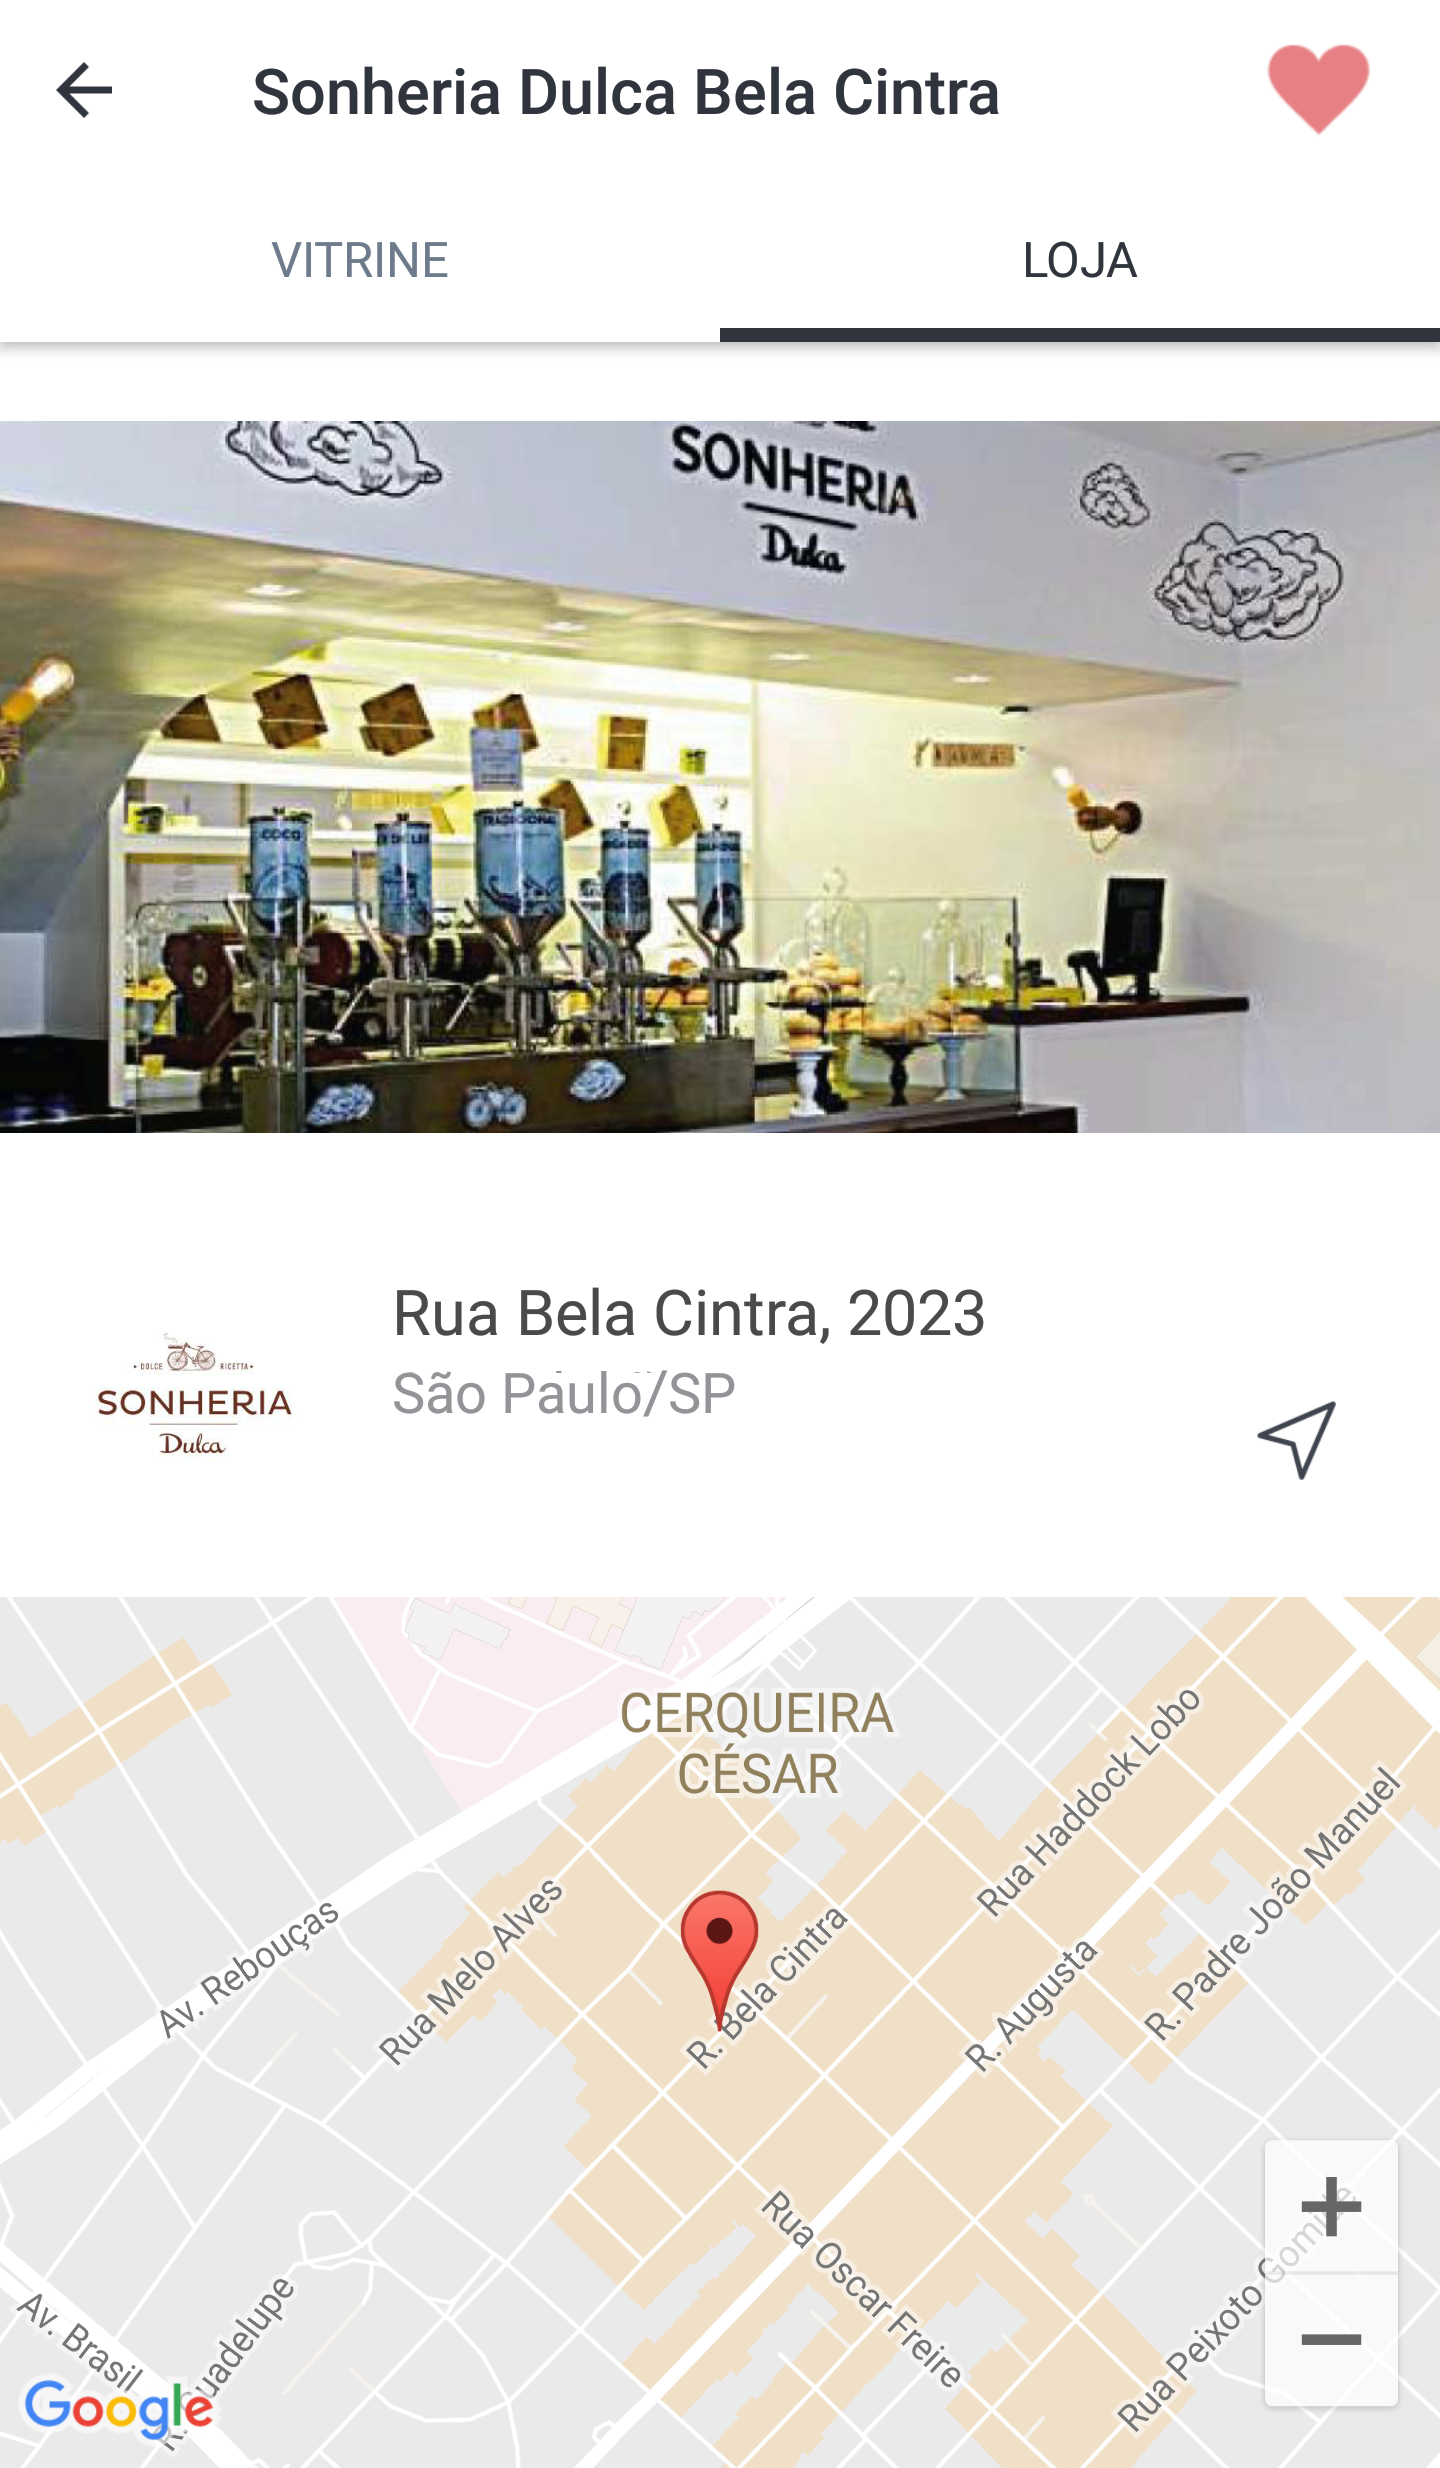
\includegraphics[scale=0.13]{img/info_parceiros}}
\label{fig:info_parceiros}
\caption* {Fonte: Aplicativo Beeconnect}
\end{figure}

\section{Testar Hipóteses}
\label{cha:testar_hipoteses}
Durante o mês de março a equipe focou em realizar os testes o mais rápido possível. 

\subsection{Teste da hipótese 1}
\label{cha:teste_1}
Para testar a hipótese 1 foi organizado um mutirão de vendas durante uma segunda-feira que focou na região da Paulista entre os metrôs Trianon-Masp e Consolação devido a proximidade com o escritório. Onze membros da Beeconnect participaram do mutirão organizados em cinco grupos, quatro duplas e um trio, cada grupo deveria percorrer uma das áreas, ilustradas na \autoref{fig:area_mutirao}.

\begin{figure}[H]
\caption{Área coberta pelo mutirão de vendas}
\centerline{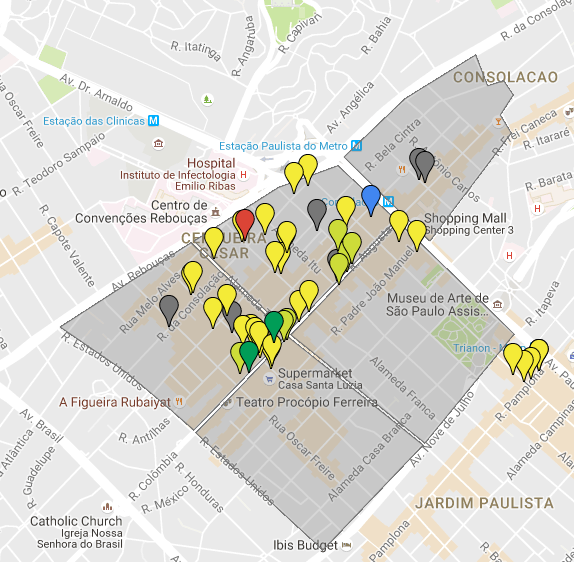
\includegraphics[scale=0.25]{img/area_mutirao}}
\label{fig:area_mutirao}
\caption* {Fonte: Elaborado pelo autor através da ferramenta do Google Maps}
\end{figure}

Durante o mutirão de vendas os membros da equipe tentaram vender primeiro o plano mensal com beacons que custava R\$99 por mês por beacon por loja, caso não houvesse interesse o membro oferecia o plano sem beacon que custava R\$49 por mês por loja. A equipe também carregava uma apresentação impressa, exemplo de slide na \autoref{fig:apresentacao_vendas_bc}, da Beeconnect para deixar com os funcionários da loja caso o dono não estivesse presente.

\begin{figure}[H]
\caption{Exemplo de slide da Apresentação de Vendas}
\centerline{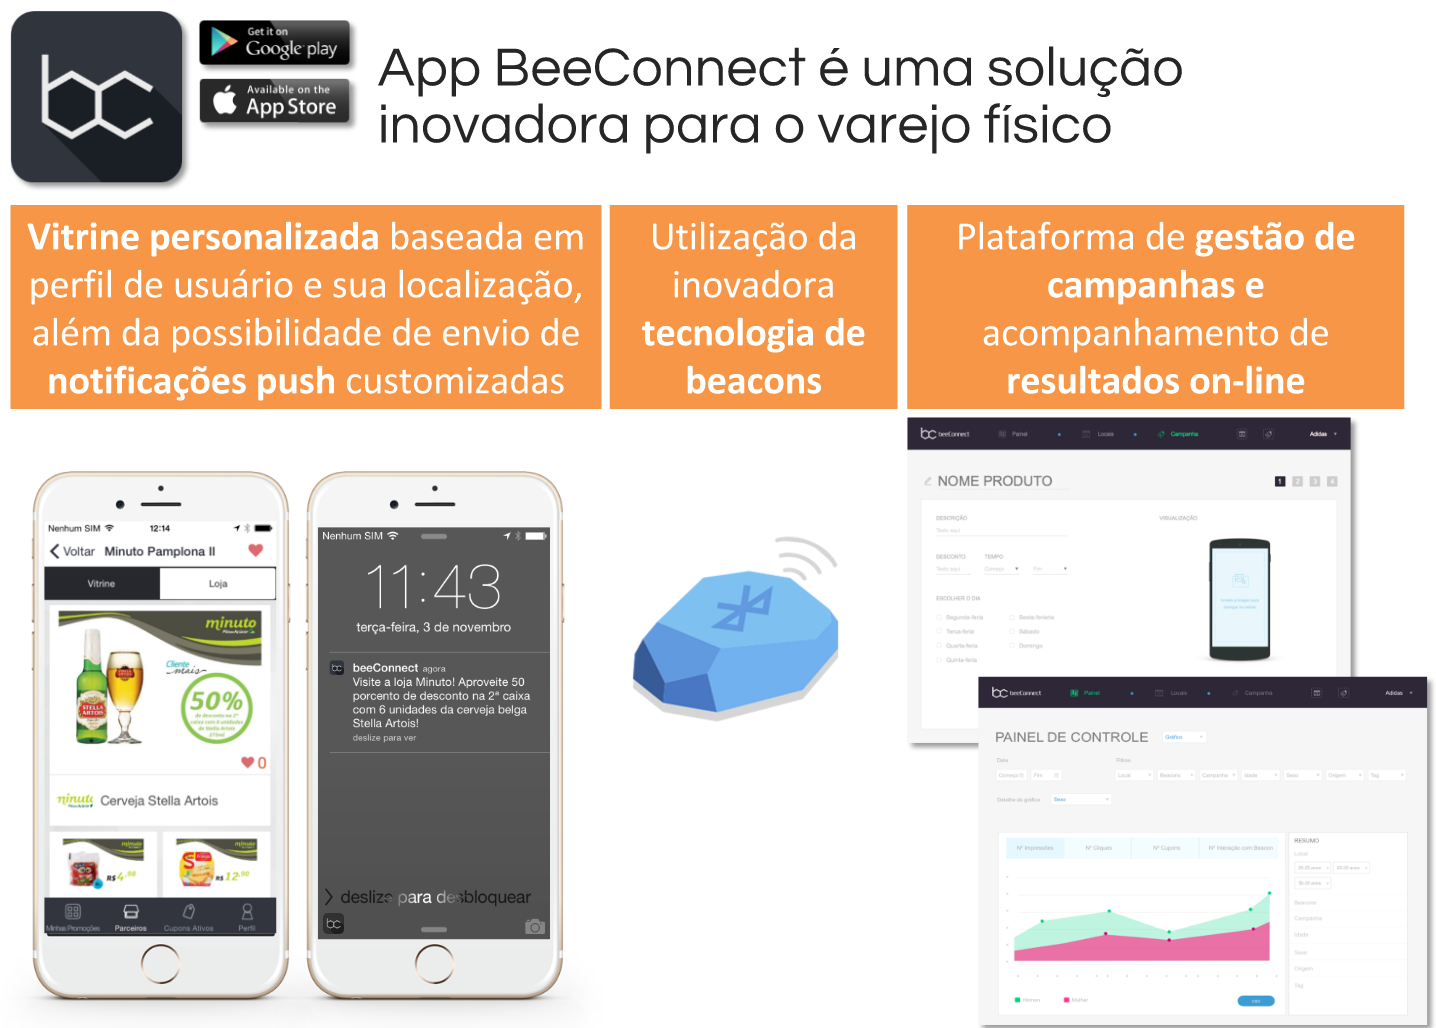
\includegraphics[width=0.8\textwidth]{img/apresentacao_vendas_bc}}
\label{fig:apresentacao_vendas_bc}
\caption* {Fonte: Material de vendas da Beeconnect}
\end{figure}

\subsection{Teste da hipótese 2}
\label{cha:teste_2}
Para o teste da hipótese 2, que foi realizado dois dias após o mutirão de vendas, o time comercial da startup ligou para todos os varejistas que estavam participando no aplicativo para perguntar se eles estavam dispostos a dar pelo menos um desconto exclusivo no aplicativo.

\subsection{Teste da hipótese 3}
\label{cha:teste_3}
O teste da hipótese 3 foi realizado dois dias após a realização do teste 2, ou seja, em uma sexta-feira. A equipe da Beeconnect criou um post pago no Facebook, conforme mostra a \autoref{fig:post_sonheria}, com a melhor oferta disponível no aplicativo na época, "50\% de desconto na compra do segundo sonho" na Sonheria Dulca. Na campanha de marketing a equipe mirou no público que havia dado curtir na página do Facebook da Sonheria. A campanha rodou por 1 dia por motivos de orçamento.

\begin{figure}[H]
\caption{Post Facebook Sonheria Dulca}
\centerline{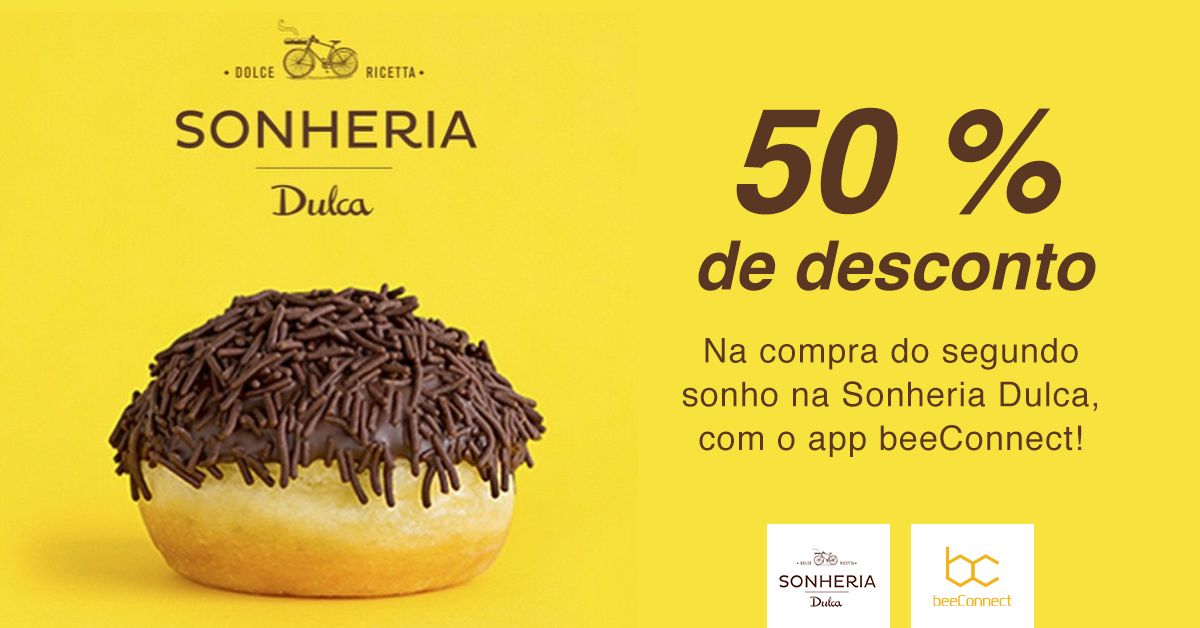
\includegraphics[width=0.8\textwidth]{img/post_sonheria}}
\label{fig:post_sonheria}
\caption* {Fonte: Material de marketing da Beeconnect}
\end{figure}

\subsection{Teste da hipótese 4}
\label{cha:teste_4}
Para o teste da hipótese 4, que começou um dia após a realização do teste 3, utilizou-se do monitoramento desenvolvido dentro do aplicativo para analisar o comportamento dos usuários que baixaram o app através do post feito no Facebook. O objetivo era ver quantos usuários únicos iriam gerar cupom durante a primeira semana de experiência do aplicativo.

\subsection{Teste da hipótese 5}
\label{cha:teste_5}
Para testar a hipótese 5 foi realizado após uma semana em relação ao teste 4 com intuito de fazer uma análise de coorte do grupo de usuários que foi impactado pelo post feito no Facebook. Analisou-se quantos usuários que geraram cupom na semana anterior também geraram cupom naquela semana.

\subsection{Teste da hipótese 6}
\label{cha:teste_6}
O teste da hipótese 6 foi realizado em paralelo com os teste 4 e 5. Através do monitoramento feito no aplicativo foi possível analisar quantos usuários únicos acessaram a tela de informações da Sonheria Dulca, ilustrada na \autoref{fig:info_parceiros}.

\section{Analisar Resultados e Repetir Ciclo}
\label{cha:analisar_resultados}
Essa seção apresenta quais foram os resultados obtidos durante a fase de testes assim como faz uma análise desses resultados.

\subsection{Resultado do Teste da hipótese 1}
\label{cha:resultado_1}
Durante esse teste foram visitadas 70 lojas, sendo que 10 decidiram fazer parte do aplicativo, ou seja, pouco mais que 14\% das lojas foram convertidas, como mostra a \autoref{tab:resultado_1}. Dado que a porcentagem esperada de lojas convertidas era de 10\%, pode-se dizer que a Beeconnect passou no teste.
\begin{table}[H]
\centering
\caption{Resultado do teste da hipótese 1}
\label{tab:resultado_1}
\begin{tabular}{|c|c|c|c|}
\hline
Número de Lojas Visitadas & Número de Lojas Convertidas & Resultado & Esperado          \\ \hline
70                        & 10                          & 14\%      & \textgreater 10\% \\ \hline
\end{tabular}
\caption* {Fonte: Elaborado pelo autor}    
\end{table}

\subsection{Resultado do Teste da hipótese 2}
\label{cha:resultado_2}
Ao ligar para os varejistas, os vendedores da Beeconnect conseguiram que 12 das 28 lojas parceiras no momento disponibilizassem descontos exclusivos para o aplicativo, ou seja, pouco mais que 42\%, como mostra a \autoref{tab:resultado_2}. Nesse teste também pode-se concluir que a startup passou no teste dado que seu resultado de 42\% foi maior que o esperado de 40\%.
\begin{table}[H]
\centering
\caption{Resultado do teste da hipótese 2}
\label{tab:resultado_2}
\begin{tabular}{|c|c|c|c|}
\hline
Lojas com Desconto Exclusivo & Lojas Parceiras & Resultado   & Esperado          \\ \hline
12                       	  & 28              & 42.8\%      & \textgreater 40\% \\ \hline
\end{tabular}
\caption* {Fonte: Elaborado pelo autor}    
\end{table}

\subsection{Resultado do Teste da hipótese 3}
\label{cha:resultado_3}
O post no Facebook feito para a campanha da Sonheria rendeu 90 downloads do aplicativo, sendo visto por 55440 vezes, o que deu uma conversão de 0,23\%, que ficou bem abaixo do esperado de 1\%, referenciado na \autoref{tab:resultado_3_1}. Cada download custou cerca de R\$ 4,43, bem acima que o esperado de R\$1,00, como visto na \autoref{tab:resultado_3_2}. Portanto, os dois resultados do teste com o post no Facebook foram bem insatisfatórios para a Beeconnect.
\begin{table}[H]
\centering
\caption{Resultado 1 do teste da hipótese 3}
\label{tab:resultado_3_1}
\begin{tabular}{|c|c|c|c|}
\hline
Downloads & Alcance & Conversão & Conversão Esperada \\ \hline
90                       & 55440 &  0.23\%     & \textgreater 0.5\% \\ \hline
\end{tabular}
\caption* {Fonte: Elaborado pelo autor}    
\end{table}

\begin{table}[H]
\centering
\caption{Resultado 2 do teste da hipótese 3}
\label{tab:resultado_3_2}
\begin{tabular}{|c|c|c|}
\hline
Custo por Download & Custo por Download Esperado \\ \hline
R\$4,43          & \textless R\$1,00 \\ \hline
\end{tabular}
\caption* {Fonte: Elaborado pelo autor}    
\end{table}


\subsection{Resultado do Teste da hipótese 4}
\label{cha:resultado_4}
Dos 90 usuários que baixaram o aplicativo através do Post do Facebook criado para a hipótese 3, 11 conseguiram gerar ao menos um cupom na primeira semana de uso do aplicativo, uma conversão de pouco mais que 12\%. Portanto, o resultado foi positivo para empresa dado que o esperado era que 10\% dos usuários gerassem cupons, como mostra a \autoref{tab:resultado_4}.
\begin{table}[H]
\centering
\caption{Resultado do teste da hipótese 4}
\label{tab:resultado_4}
\begin{tabular}{|c|c|c|c|}
\hline
Usuários & Usuários Únicos com Cupom & Conversão & Conversão Esperada \\ \hline
90       & 11  & 12.2\%   & \textgreater 10\% \\ \hline
\end{tabular}
\caption* {Fonte: Elaborado pelo autor}    
\end{table}

\subsection{Resultado do Teste da hipótese 5}
\label{cha:resultado_5}
Dos 11 usuários que geraram pelo menos um cupom na primeira semana de uso do aplicativo, 3 geraram pelo menos um cupom na segunda semana do aplicativo, pouco mais de 27\%, conforme mostra a \autoref{tab:resultado_5}. Como mencionado anteriormente, o resultado esperado era de 25\%, portanto a empresa teve um resultado positivo quanto a um teste de retenção.
\begin{table}[H]
\centering
\caption{Resultado do teste da hipótese 5}
\label{tab:resultado_5}
\begin{tabular}{|c|c|c|c|}
\hline
Usuários cupom semana 1 & Usuários cupom semana 2 & Resultado & Esperado \\ \hline
11       & 3  & 27.2\%   & \textgreater 25\% \\ \hline
\end{tabular}
\caption* {Fonte: Elaborado pelo autor}    
\end{table}

\subsection{Resultado do Teste da hipótese 6}
\label{cha:resultado_6}
Quanto ao teste de consultas à tela de informações do parceiro, dos 90 usuários que baixaram o aplicativo, 15 consultaram ao menos uma vez essa tela durante as duas semanas de monitoramento, cujo resultado dá aproximadamente 17\%, muito abaixo dos 30\% esperados, como mostra a \autoref{tab:resultado_6}. Pode-se concluir então que a tela com a funcionalidade de informações do parceiro foi em vão e que talvez o tempo dos desenvolvedores poderia ser focado em outras funcionalidades mais importantes. 

\begin{table}[H]
\centering
\caption{Resultado do teste da hipótese 6}
\label{tab:resultado_6}
\begin{tabular}{|c|c|c|c|}
\hline
Usuários & Usuários que consultaram a tela de informações & Resultado & Esperado \\ \hline
90       & 15  & 16.7\%   & \textgreater 30\% \\ \hline
\end{tabular}
\caption* {Fonte: Elaborado pelo autor}    
\end{table}

\section{Listar Lições Aprendidas do Primeiro Ciclo}
\label{cha:listar_licoes_aprendidas}
Durante o mutirão de vendas a equipe notou que se tivesse levado uma câmera digital ou levado um cartão de memória para conseguir as fotos dos produtos de uma loja seria muito mais rápido de integrar com novos varejistas.
O fato de levar os beacons para apresentá-los no mutirão foi um fator relevante para mostrar o diferencial do produto. As equipes que não levaram o aparelho tiveram um desempenho pior que as demais.
Para que os varejistas entendessem melhor sobre o que aplicativo estava tentando oferecer os membros utilizaram termos como "o aplicativo é como um jornal do bairro no celular", "o aplicativo é uma extensão da vitrine física no celular", "trabalhamos com marketing digital". Tal estratégia pareceu funcionar bem.

Todos as lojas que estavam no aplicativo não estavam pagando pelo uso do serviço. Uma maneira de alavancar a parceria foi pedir para que as lojas postassem em suas páginas do Facebook dizendo que elas estavam fazendo parte da Beeconnect, conforme ilustrado na \autoref{fig:paulista_burger}.

\begin{figure}[H]
\caption{Post da Página do Paulista Burger}
\centerline{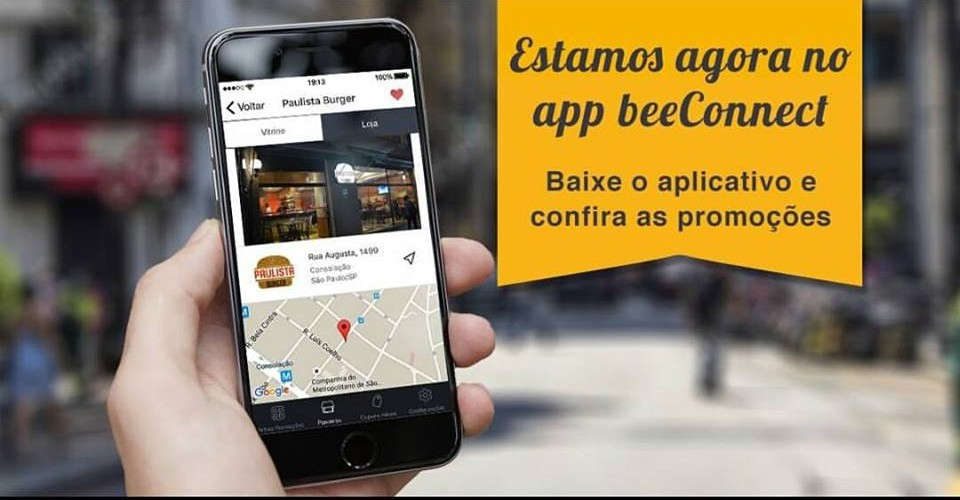
\includegraphics[width=0.8\textwidth]{img/paulista_burger}}
\label{fig:paulista_burger}
\caption* {Fonte: https://www.facebook.com/paulistaburger/}
\end{figure}

A publicação paga no \textit{Facebook} tendo como público-alvo uma determinada página não pareceu funcionar tão bem, a conversão foi relativamente alta se comparar com a média de mercado. Entretanto, o alto custo por download deixa inviável tal iniciativa.

Outro aprendizado é de tentar validar se há uma demanda real por uma determinada funcionalidade no aplicativo, como aconteceu com o item da hipótese 6, a tela de informações do parceiro. Dado que o time de desenvolvimento tem um tempo escasso e valioso o foco deve ser alocar os recursos do time só em funcionalidades que claramente geram valor para seus usuários.

Os resultados quanto a retenção dos clientes foi melhor que o esperado, entretanto deve-se medir ainda mais a retenção no decorrer de meses. Dados os resultados dos testes o autor decidiu iterar pelo ciclo mais uma vez para aprender mais sobre o modelo de negócio da startup, principalmente na questão se os clientes estariam dispostos a pagar pelo serviço prestado.

\section{Mapear estado atual da startup 2}
\label{cha:mapear_estado_2}
A partir da evolução na compreensão do modelo de negócio da Beeconnect a equipe decidiu elaborar um novo Canvas de Modelo Negócio, referenciado na \autoref{fig:canvas_beeconnect_2}, para que ficasse mais fácil de visualizar os novos aprendizados. Só foram feitos alguns ajustes em relação ao canvas inicial nos blocos:

\begin{itemize}
\item Proposta de Valor: houve um ajuste na formulação dos descontos exclusivos para "Cupons de descontos exclusivos". Além disso, houve a remoção do item "Fácil acesso a informação das lojas físicas", porque devido aos testes executados no primeiro ciclo ficou claro que tal funcionalidade não gerava valor para os usuários.
\item Segmentos de Clientes: A modificação feita foi de "Compradores que gostam de descontos" para "Compradores de lojas físicas". O motivo dessa mudança foi porque o aplicativo não quis focar nos compradores de lojas virtuais, e também dado que o aplicativo também tem a função de ser um panfleto digital, aumentar o escopo para compradores de lojas físicas pode aumentar a base de usuários.
\item Fluxo de Receita: Dada as conversas com os próprios varejistas muitos perguntavam se o usuário teria que pagar alguma quantia para usufruir do aplicativo. A equipe decidiu deixar claro no canvas que o usuário não iria desembolsar nada para utilizar o app.
\end{itemize}

\begin{figure}[H]
\caption{Canvas de Modelo de Negócio após testes}
\centerline{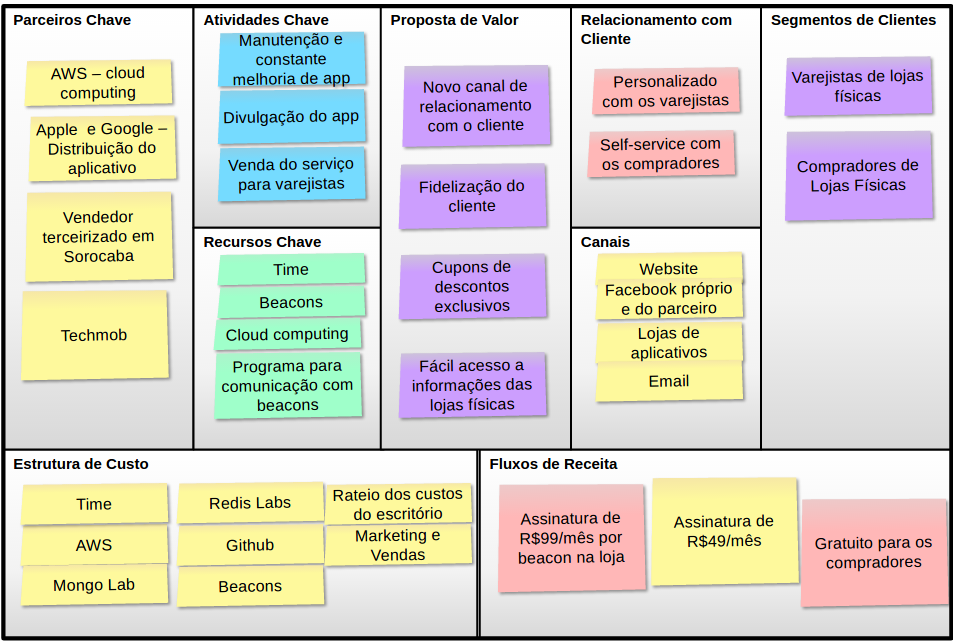
\includegraphics[width=0.8\textwidth]{img/canvas_beeconnect_2}}
\label{fig:canvas_beeconnect_2}
\caption* {Fonte: Elaborado pelo autor}
\caption* {Legenda: As caixas com cores diferentes em relação ao seu bloco são as que sofreram alterações}
\end{figure}

\section{Gerar hipóteses sobre a proposta de valor da empresa 2}
\label{cha:gerar_hipoteses_ 2}
Uma vez que as seis hipóteses elaboradas no ciclo anterior foram respondidas e o canvas do estado atual foi elaborado, o autor se encontrou novamente com o seu orientador para gerar novas hipóteses sobre a proposta de valor. Os dois concordaram que a próxima etapa seria provar o valor do produto para os lojistas e comprovar se os varejistas estavam dispostos a pagar pelo serviço. Então a sétima hipótese elaborada no decorrer do trabalho de conclusão de curso foi:
\begin{itemize}
\item Hipótese 7: \textbf{Os varejistas estão dispostos a pagar pelo serviço}.
\end{itemize}


\section{Desenhar Testes de Hipóteses 2}
\label{cha:desenhar_hipoteses_2}
Após a formulação da hipótese foi feita a estruturação para que tal suposição fosse testada corretamente.

\subsection{Hipótese 7}
\label{cha:hipotese_7}
Para provar que os varejistas estavam dispostos a pagar pelo serviço do aplicativo Beeconnect antes seria necessário provar para os varejistas que o serviço deveras gerava um retorno positivo. Para isso o autor elaborou uma fórmula básica para provar tal hipótese:

\[[(NC * (PC - D)) + (VR * (PC - D))] > PS\]

Onde: 
\begin{itemize}
\item NC: é o numero de novos clientes.
\item PC: é o preço cheio de um produto, ou seja, o valor original de um produto.
\item D: é o valor do desconto aplicado ao produto.
\item VR: é o número de vendas recursivas, isto é o número de compras repetidas feitas por usuários do aplicativo Beeconnect.
\item PS: é o preço do serviço cobrado pela Beeconnect, explicado na \autoref{cha:fluxos_de_receita_canvas_bc_1}.
\end{itemize}

Então seria necessário pelo menos uma loja disposta a fazer uma promoção disponibilizando um cupom exclusivo para testar tal hipótese.
\section{Testar Hipóteses 2}
\label{cha:testar_hipoteses_2}

\subsection{Teste da hipótese 7}
\label{cha:teste_hipotese_7}
A equipe acabou conseguindo três lojas, sendo duas do setor alimentício e uma do setor vestuário. Para o teste com as duas lojas do setor alimentício, uma gelateria e uma sonheria, a equipe organizou um mutirão de marketing, que cobria a região entre as duas lojas, que ficavam localizadas na região dos Jardins entre as ruas Bela Cintra e Augusta, como mostra a \autoref{fig:mutirao_mkt}.
\begin{figure}[H]
\caption{Região coberta pelo mutirão de marketing}
\centerline{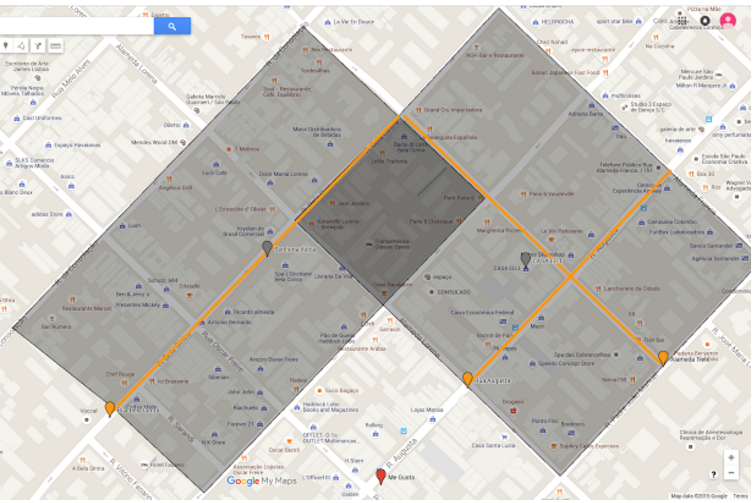
\includegraphics[width=0.8\textwidth]{img/mutirao_mkt}}
\label{fig:mutirao_mkt}
\caption* {Fonte: Elaborado pelo autor}
\end{figure}

Durante o mutirão a equipe da Beeconnect distribuiu panfletos para divulgar o aplicativo, distribuiu também alguns chaveiros com a marca da empresa e também carregou alguns balões com gás hélio para chamar mais atenção do publico que passava pela rua. A intenção era que o público baixasse o app na hora e fosse visitar as lojas que estavam disponibilizando descontos exclusivos no aplicativo.

A gelateria disponibilizou a oferta de \textit{"Gelato médio de R\$15 por R\$11"}. A oferta disponibilizada pela sonheria foi \textit{"Compre 2 sonhos pague 1"} e por fim a loja de vestuário estava ofertando um sapatênis \textit{"De R\$299 por R\$199"}.

\section{Analisar Resultados e Repetir Ciclo 2}
\label{cha:analisar_resultados_2}
Os resultados foram medidos ao longo de uma semana após a realização do mutirão de marketing.

\subsection{Resultado do Teste da hipótese 7}
\label{cha:resultado_7}
Após a realização dos testes para confirmar se os varejistas estavam dispostas a pagar pelo serviço, o autor então analisou o resultado de cada uma das lojas.

\subsubsection{Gelateria Casa Elli}
\label{cha:resultado_casa_elli}
O resultado na gelateria Casa Elli foi satisfatório, foram gerados 30 cupons sendo utilizados 26, onde 24 novos clientes que acabaram comprando o gelato médio cujo preço era de R\$15, como mencionado na \autoref{cha:teste_hipotese_7}, mas graças ao desconto pelo aplicativo Beeconnect saiu por R\$11. Os outros dois cupons foram utilizados por usuários antigos do aplicativo, ou seja, se encaixaram nas vendas recursivas como mostra a \autoref{tab:resultado_7_casa_elli_a}.

\begin{table}[H]
\centering
\caption{Resultado do teste 7 na Gelateria Casa Elli}
\label{tab:resultado_7_casa_elli_a}
\begin{tabular}{|c|c|c|c|}
\hline
Novos Clientes & Preço Cheio & Desconto & Vendas Recursivas \\ \hline
24             & 15          & 4        & 2   \\ \hline
\end{tabular}
\caption* {Fonte: Elaborado pelo autor}    
\end{table}

Aplicando os números acima na fórmula mencionada na \autoref{cha:hipotese_7}, surge o resultado abaixo:
\[[(24 * (15 - 4)) + (2 * (15 - 4))] = 286\]

Como a gelateria estava usufruindo da tecnologia de beacons, sua mensalidade custaria R\$99/mês que, quando comparada com resultado de R\$286 advindo do aplicativo Beeconnect em apenas uma semana, pode-se analisar que seria um bom investimento, como mostra a \autoref{tab:resultado_7_casa_elli_b}. 

\begin{table}[H]
\centering
\caption{Análise do teste 7 na Gelateria Casa Elli}
\label{tab:resultado_7_casa_elli_b}
\begin{tabular}{|c|c|c|}
\hline
Resultado & Mensalidade & Retorno do Investimento \\ \hline
286             & 99          &   2.88 \\ \hline
\end{tabular}
\caption* {Fonte: Elaborado pelo autor}    
\end{table}

Apesar do resultado positivo tanto para a gelateria quanto para a Beeconnect, a dona da loja ainda não estava disposta a pagar pelo serviço, ela gostaria de mais tempo para decidir se estava disposta a pagar a quantia. Entretanto, ela disse que utilizaria a plataforma para subir mais campanhas e que daria mais feedbacks para que a equipe conseguisse melhorar ainda mais o produto.

Tal comportamento foi encarado de maneira bastante inesperada pela equipe do aplicativo, que esperava que a varejista já assinasse algum tipo de contrato dizendo que iria pagar pelo serviço disponibilizado pela Beeconnect.

\subsubsection{Sonheria Dulca}
\label{cha:resultado_sonheria_dulca}
O resultado na Sonheria Dulca também foi positivo, foram gerados 21 cupons sendo 19 deles utilizados, onde 18 foram utilizados por novos clientes e 1 foi usufruído por um cliente antigo. Como mencionado anteriormente, a oferta disponiblizada foi de "Compre 2 sonhos pague 1", na época cada sonho custava R\$10, ou seja, o preço cheio seria de R\$20 e o desconto seria de R\$10, como mostra a \autoref{tab:resultado_7_sonheria_dulca_a}

\begin{table}[H]
\centering
\caption{Resultado do teste 7 na Sonheria Dulca}
\label{tab:resultado_7_sonheria_dulca_a}
\begin{tabular}{|c|c|c|c|}
\hline
Novos Clientes & Preço Cheio & Desconto & Vendas Recursivas \\ \hline
18             & 20          & 10        & 1   \\ \hline
\end{tabular}
\caption* {Fonte: Elaborado pelo autor}    
\end{table}

Aplicando os números acima na fórmula mencionada na \autoref{cha:hipotese_7}, surge o resultado abaixo:
\[[(18 * (20 - 10)) + (1 * (20 - 10))] = 190\]

Assim como a Gelateria, a Sonheria também utilizava a tecnologia de beacons, portanto a mensalidade seria de R\$99/mês. O resultado de R\$190 sem contar com as vendas casadas de água e café foi positivo para a loja, como apresenta a \autoref{tab:resultado_7_sonheria_dulca_b}.

O time da Beeconnect ficou bastante preocupado em virtude da falta de interesse dos varejistas resolverem pagar pelo serviço apesar dos resultados positivos. Seria necessário no próximo ciclo de testes de hipótese algum tipo de mudança para que os varejistas não tivessem como negar o pagamento do serviço.

\begin{table}[H]
\centering
\caption{Análise do teste 7 na Sonheria Dulca}
\label{tab:resultado_7_sonheria_dulca_b}
\begin{tabular}{|c|c|c|}
\hline
Resultado & Mensalidade & Retorno do Investimento \\ \hline
190             & 99          &   1.91 \\ \hline
\end{tabular}
\caption* {Fonte: Elaborado pelo autor}    
\end{table}

Os donos da loja também não se mostraram interessados em pagar pela utilização do serviço e também disseram que não estavam dispostos a utilizar a plataforma por conta própria pois não possuíam uma pessoa disponível para criar as campanhas e administrá-las.

\subsubsection{Tisu Store}
\label{cha:resultado_tisu_store}
No caso da Tisu Store, a oferta do sapatênis com desconto de R\$100 teve 3 cupons gerados, entretanto, não houve utilização desses cupons. Portanto, o resultado foi bem insatisfatório, como mostram a \autoref{tab:resultado_7_tisu_store_a} e a \autoref{tab:resultado_7_tisu_store_b}.


\begin{table}[H]
\centering
\caption{Resultado do teste 7 na Tisu Store}
\label{tab:resultado_7_tisu_store_a}
\begin{tabular}{|c|c|c|c|}
\hline
Novos Clientes & Preço Cheio & Desconto & Vendas Recursivas \\ \hline
0             & 299          & 100        & 0 \\  \hline
\end{tabular}
\caption* {Fonte: Elaborado pelo autor}    
\end{table}

Aplicando os números acima na fórmula mencionada na \autoref{cha:hipotese_7}, surge o resultado abaixo:
\[[(0 * (299 - 100)) + (0 * (299 - 100))] = 0\]

\begin{table}[H]
\centering
\caption{Análise do teste 7 na Tisu Store}
\label{tab:resultado_7_tisu_store_b}
\begin{tabular}{|c|c|c|}
\hline
Resultado & Mensalidade & Retorno do Investimento \\ \hline
0             & 99          &   0 \\ \hline
\end{tabular}
\caption* {Fonte: Elaborado pelo autor}    
\end{table}

Como era de se esperar com esse resultado tão ruim o dono da loja não mostrou nenhum interesse em pagar pelo serviço e também disse que não iria utilizar a plataforma por conta própria. 

\section{Listar Lições Aprendidas do Segundo Ciclo}
\label{cha:listar_licoes_aprendidas_segundo_ciclo}
O segundo ciclo buscou responder se os lojistas iram pagar pelo uso do serviço do aplicativo. Apesar de nenhum parceiro ter se disposto a desembolsar uma quantia mensal para usufruir da plataforma, a equipe tirou aprendizados importantes desse teste.

O primeiro aprendizado foi que o setor de comidas e bebidas apresentou-se como um nicho mais fácil de conseguir novos usuários para o aplicativo. Dado que o valor médio do produto é mais baixo, fica mais fácil o primeiro contato do usuário com o aplicativo, o cliente já vê o benefício muito mais rápido.

A equipe pensou que talvez um outro meio de conseguir que os varejistas paguem talvez seja cobrar também uma taxa a mais pela administração de campanhas no aplicativo. Isso se justifica pelo motivo que muitos não queriam pagar pela mensalidade pelo fato da plataforma ser auto gerida e eles não queriam gastar tempo com gerenciamento da plataforma.

\section{O Fim da Beeconnect}
\label{cha:fim_da_beeconnect}
Infelizmente não foi possível uma execução sucessiva de outros ciclos para testar novas hipóteses sobre o modelo de negócio da Beeconnect. O conselho da holding TM decidiu fechar o projeto com a justificativa que apesar dos aprendizados adquiridos com a Beeconnect, a startup ainda não havia provado o seu modelo de negócio e não parecia haver no horizonte que a situação iria mudar rapidamente.

O sentimento amargo de derrota foi horrível, todo o time ficou desmotivado com a notícia. O grande problema é que não houve um aviso prévio por parte do conselho da holding, a decisão foi repentina, então o time não saiu com um sentimento de dever cumprido, de que tinha tentado com todas as forças todas as alternativas e não estava preparado para tal notícia. Também houve uma sensação no ar que iriam haver demissões.

Apesar das más notícias, o time da startup foi mantido, mas cada um foi suprir uma função diferente dentro da TM. Dois membros foram ajudar no time de ciência de dados na RM. Três membros foram ajudar no time que desenvolve o software que faz mostrar as propagandas da RM nos aplicativos de parceiros. Três membros foram auxiliar no time da BL para construir a plataforma de visualização de análise de dados. Outros dois foram auxiliar no time de vendas da RM para conseguir mais desenvolvedores para a plataforma. O autor ajudou por um tempo na RM integrando com novos parceiros para conseguir disponibilizar as propagandas RM em novos aplicativos, depois o desafio que foi lhe proposto foi de ajudar a desenvolver o banco de dados da BL.

O fim da Beeconnect de fato chocou a todos que estavam fazendo parte dessa jornada, porque toda equipe acreditava bastante no projeto que poderia revolucionar o varejo de lojas físicas. A empresa era composta por pessoas incríveis e competentes, que por falta da utilização de uma metodologia voltada para desenvolvimento de startups acabou sucumbindo a meramente a um status de projeto engavetado.
%!TEX root = index.tex
\chapter{Conclusão}

\section{Discussão} % (fold)
\label{sec:discussao}
Por que a Beeconnect não foi para frente? O que deu errado?

Desde o princípio a ideia que norteou a Beeconnect foi o uso da tecnologia de beacons. Os membros do board da Techmob foram à Mobile World Conference em 2014 e ficaram encantados com essa tecnologia, que prometia alta precisão de localização indoor. Eles queriam utilizá-los mas não sabiam como. O problema é que esse processo de desenvolvimento da startup pulou uma série de etapas importantes para a geração e desenvolvimento do modelo de negócio. O beacon no caso deveria ser um meio e não um fim.

Pelo fato de ser originada a partir da Revmob, a Beeconnect ficou com a ideia muito rígida de que propaganda era o caminho a ser trilhado. Por esse fato a equipe perdeu no início cerca de um mês desenvolvendo algo que no final provou ser inútil. Faltou benchmarking e o entendimento do mercado.

Durante o desenvolvimento do aplicativo iShop, que posteriormente foi renomeado para Beeconnect, a equipe ficou muito distante do consumidor final. Faltou coleta de feedbacks e iteração em cima deles. Com tais dados ficaria muito mais fácil de debater em cima do produto ao invés de divagar sobre o que o cliente iria gostar.

Faltou criatividade para a validação da hipótese do aplicativo. Ao invés de gastar seis meses quase quinhentos mil reais em equipe para desenvolvimento seria muito mais simples desenvolver um vídeo, um simples site e algum dinheiro em publicidade no Facebook para que algumas hipóteses fossem validadas rapidamente.

O modelo de negócio era totalmente diferente dos outros modelos da holding. A BCFG é B2C, a Revmob é B2B e a Beluga é B2B, enquanto a Beeconnect é B2B2C. A única sinergia era quanto ao conhecimento em desenvolvimento de servidores. Apesar da BCFG ter desenvolvido uma série de jogos para Android e iOS os desenvolvedores desses jogos não estavam mais presentes então não houve compartilhamento de conhecimento para a programação de aplicativos nessas plataformas.

Um dos maiores problemas para a Beeconnect foi ter que lidar com as duas pontas, as lojas físicas e os usuários dos aplicativos. Modelos de negócio desse tipo demandam muito capital porque para ele funcionar bem seriam necessários muitos usuários e muitas lojas, o que demanda dinheiro e muito tempo. Para que a empresa tivesse uma sobrevida provavelmente a captação de investimento seria a saída, o empecilho é que a holding não gosta de investimentos externos por problemas passados.

Quanto a organização da empresa houve também diversos erros. Foram contratados mais funcionários do que poderia ser absorvido. Isso ocasionou um transtorno no processo de desenvolvimento pois a pessoa que mais produzia tinha que parar para ensinar três pessoas. Outro erro foi ter criado a startup como uma Sociedade em Conta de Participação. Basicamente, quem saiu da Revmob e foi para a Beeconnect abriu mão de ações da Revmob para ter a promessa de ganhar mais ações da Beeconnect. Isso ocasionou alguns problemas como falta de empatia por parte das outras pessoas da holding que não viam tanto valor em ajudar a nova startup visto que eles não ganhariam tanta participação no processo. Além disso, essa estrutura era mais rígida e não permitia mudanças rápidas de recursos entre as empresas do grupo Techmob.

A falta de experiência tanto na programação quanto na parte de negócios foi também um grande empecilho para o sucesso da empresa. Ninguém da equipe tinha criado uma conta de desenvolvedor na Apple. Esse processo é demorado e custoso. Além disso, a empresa de Cupertino é muito rigorosa no processo de avaliação de seus aplicativos. O app de iOS atrasou em quase 2 meses por tais motivos. A cada mês mais e mais capital era drenado da empresa então o quanto antes o MVP fosse lançado melhor seria para iterar sobre o processo de Construir-Medir-Aprender. Outro problema foi a falta de conhecimento na hora de criar um produto novo. Ao chamar o app de iShop e fazer todo o design em cima dele para depois ter que modificar para Beeconnect tomou um tempo considerável. Tal erro custou para a equipe cerca de duas semanas, fora os honorários do advogado.

Outro erro foi ter escolhido o primeiro parceiro para o piloto. O Mc Donalds de Riviera estava muito longe do escritório da empresa. O acompanhamento do piloto é de vital importância para que a coleta de feedback seja feita da maneira correta. A distância não permitiu que a equipe estivesse presente para observar o uso do aplicativo e iterar em cima dele rapidamente.

A startup basicamente falhou por não ter seguido os princípios do Lean Startup, Design Thinking e do Desenvolvimento do Cliente. Tais princípios teriam poupado muito tempo de programação. O tempo é primordial para uma empresa cujos recursos humanos e monetários são escassos. Outro ponto fundamental é a experiência da equipe. Não havia um programador experiente para Android e iOS, desta forma gastou-se um tempo razoavelmente considerável para o desenvolvimento do aplicativo para essas duas plataformas. A política de contratação também foi falha, faltou uma busca por pessoas comprometidas, no decorrer da empresa saíram seis pessoas, o que é gigantesco para uma startup que teve no seu auge 12 pessoas, isso causa uma queda na motivação e em parte perda de conhecimento, o que é extremamente prejudicial em uma empresa nascente que deve sempre buscar estar motivada e aprendendo cada vez mais. E por fim, ter buscado um modelo negócio cujo tipo não satisfazia com o modelo que a holding busca foi totalmente inadimissível, essa falta de comunicação causou um transtorno que poderia ter sido evitado desde o início.

\section{Lições Aprendidas}
\label{sec:licoes_aprendidas}

À Techmob fica o aprendizado de uma empresa que falhou por falta de: conhecimento da literatura, política de contratação, experiência da equipe e políticas contratuais sinérgicas para os membros da holding. Além disso, tais aprendizados devem ser repassados de forma humilde para os demais funcionários da holding para que todos saibam as dificuldades enfrentadas e como não errar novamente.

Para o autor ficou aprendizado de que somente a programação e qualidade de desenvolvimento não são suficientes para que uma empresa tenha um produto de sucesso. É necessário muito mais que isso, a literatura desenvolvida durante o trabalho de formatura deve ditar o que as linhas de código devem executar. Isso tornará o trabalho muito mais ágil e fácil de ser iterado para a construção de um produto melhor e que as pessoas queiram utilizar.

Para a USP/Escola Politécnica fica a importância do fomento de criação/incubação de startups. A recomendação é permitir que os jovens arrisquem e aprendam dentro de um ambiente mais seguro. Iniciativas como o Inovalab e o Núcleo de Empreendedorismo da USP permitem um contato maior com startups e abrem novos horizontes para os universitários. Errar é um grande aprendizado, mas o mais importante de tudo é errar o quanto antes. Se os alunos conseguirem criar empresas dentro da universidade como ocorrem nas grandes instituições americanas como Stanford, MIT e Harvard será um grande passo para o futuro do empreendedorismo no Brasil.

Para o mundo fica a lição de que arriscar e buscar os sonhos é fundamental para uma vida empreendedora. É necessário falhar para aprender bastante, é durante os momentos ruins que a reflexão vem do âmago do coração empreendedor. E através dessa reflexão em conjunto com o estudo na literatura que saem novas ideias que possívelmente terão sucesso e mudarão o mundo para melhor.

%\input{cronograma}
%\pagebreak
%\input{andamento-do-projeto}
%\pagebreak
\appendix
%\input{documentacao}
%\pagebreak
%\input{sumario-final}
% ----------------------------------------------------------
% ELEMENTOS PÓS-TEXTUAIS
% ----------------------------------------------------------
\postextual
% ----------------------------------------------------------

% ----------------------------------------------------------
% Referências bibliográficas
% ----------------------------------------------------------
\bibliography{bibliografia}
\end{document}
